\chapter{Design}
\label{ch_design}
%maybe: recheck the tense (past present) of sections

This chapter presents the design of the various modules forming the laser tag system. An overview of the entire system is given in the \textit{system overview} section. The following sections, \textit{hardware design} and \textit{software design}, present the design of the modular and software components respectively.

%maybe: possibly explain why designs are so elaborate... This investigation is centred on the creation and evaluation of system modules, therefore the design descriptions have been written 

\section{System Overview}
The system overview introduces the two main subsystems, the tagger and the target.

The tagger subsystem is responsible for generating and transmitting data and the target subsystem responsible for receiving and decoding the transmitted data. The modules comprising these subsystems can be seen in figure \ref{fig:system_overview_hardware}, the dashed line shows the flow of information from the tagger subsystem to the target subsystem.

\begin{figure}[H]
	\centering
	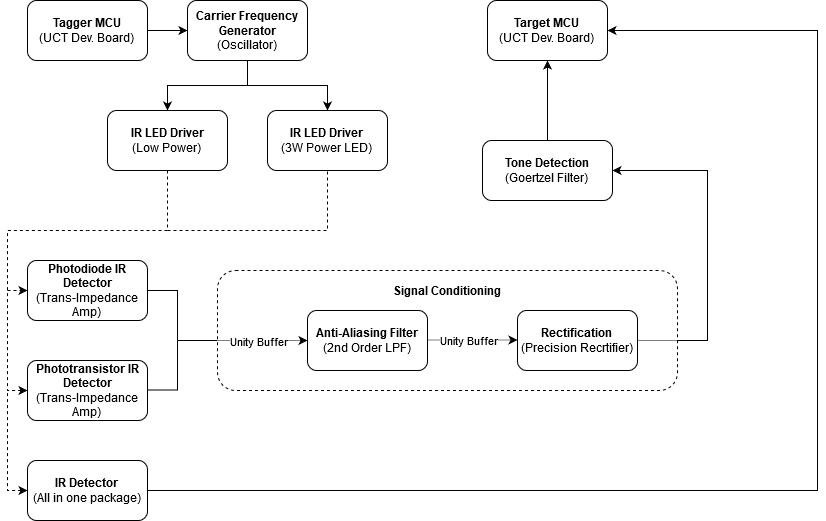
\includegraphics[width=0.9\textwidth]{figures/design/system_overview_hardware}
	\caption{Block Diagram of Hardware Modules}
	\label{fig:system_overview_hardware}
\end{figure}

\subsection{Subsystems}

\subsubsection{Tagger Subsystem}

The tagger subsystem comprises a main processor, carrier frequency generation module and two LED driver modules. It also includes the light focus system which is not included in figure \ref{fig:system_overview_hardware}.

The function of the tagger subsystem is to transmit data message via an infrared beam using a modified version of the RC-5 protocol (detailed in section \ref{sec:modified_rc5_protocol}). This operation is performed each time the user presses the designated `fire' button and the details of the transmission are presented on the LCD.


\subsubsection{Target Subsystem}

The tagger subsystem comprises a main processor, digital tone decoder, analog signal conditioning module, and three IR detector modules.

The function of the target subsystem is to detect incoming transmissions encoded in an infrared light beam and decode the message data. While active the system continuously monitors the incoming IR light and in real-time updates the LCD with received messages.

This process can be broken into 4 stages: IR detection and conversion to an analog waveform, conditioning of the analog waveform for digital signal processing, digitally processing the waveform to detect the presence of a carrier and finally decoding and displaying the encoded message. Each stage is implemented on a separate module.

\subsection{Software}

There are three main software components to the overall system.
\begin{itemize}
	\item The software operating on the tagger main processor used to encode and produce the Manchester data sequence.
	\item The software responsible for receiving and decoding the Manchester sequence on the target main processor.
	\item  The DSP algorithm operating on the tone detection module.
\end{itemize}






\section{Hardware Design}
The hardware design section presents the design of each hardware module. For each module, the \textit{functional design} header precedes a short overview of the high-level functionality of the hardware module, including the inputs and outputs. A design schematic is provided under the \textit{schematic} heading. Concerning this schematic, various design processes are presented under relevant headings. Finally, under the \textit{module realization} header, an image of the final implementation is given.


\subsection{Tagger \& Target MCUs}

\subsubsection{Functional Design}
The tagger and target microcontroller units (MCUs) handle signal encoding and decoding respectively. In the greater context of laser tag, the MCUs must perform many functions, however, in keeping with the scope of this investigation these have not been implemented.

The tagger is triggered by pulling pin 10 low, the Manchester encoded output is generated on pin 21. The target continuously monitors pin 17 for an incoming Manchester sequence.

\subsubsection{Schematic}
The schematic is available online at \href{https://gofile.io/d/Hldp7z}{https://gofile.io/d/Hldp7z}.


\subsubsection{Features}

The development board provides break-out pins for the microcontroller, 4 input buttons, an array of 8 LEDs, an LCD and a built-in st-link v2 for debugging and programming the processor.

The STM32F051C6 was chosen partly because of its integration into the UCT development board making it easily obtainable at a low price and because of the following features

\begin{itemize}
	\item Analog to digital converter (ADC) peripheral
	\item Direct memory access (DMA) peripheral
	\item Timer peripherals with multiple interrupt channels
	\item Nested vectored interrupt controller (NVIC)
\end{itemize}


\subsubsection{Module Realization}
An image of the UCT development board is shown in figure \ref{fig:module_carrier_generation}. The board is built around the STM32F051C6 microcontroller.

\begin{figure}[H]
	\centering
	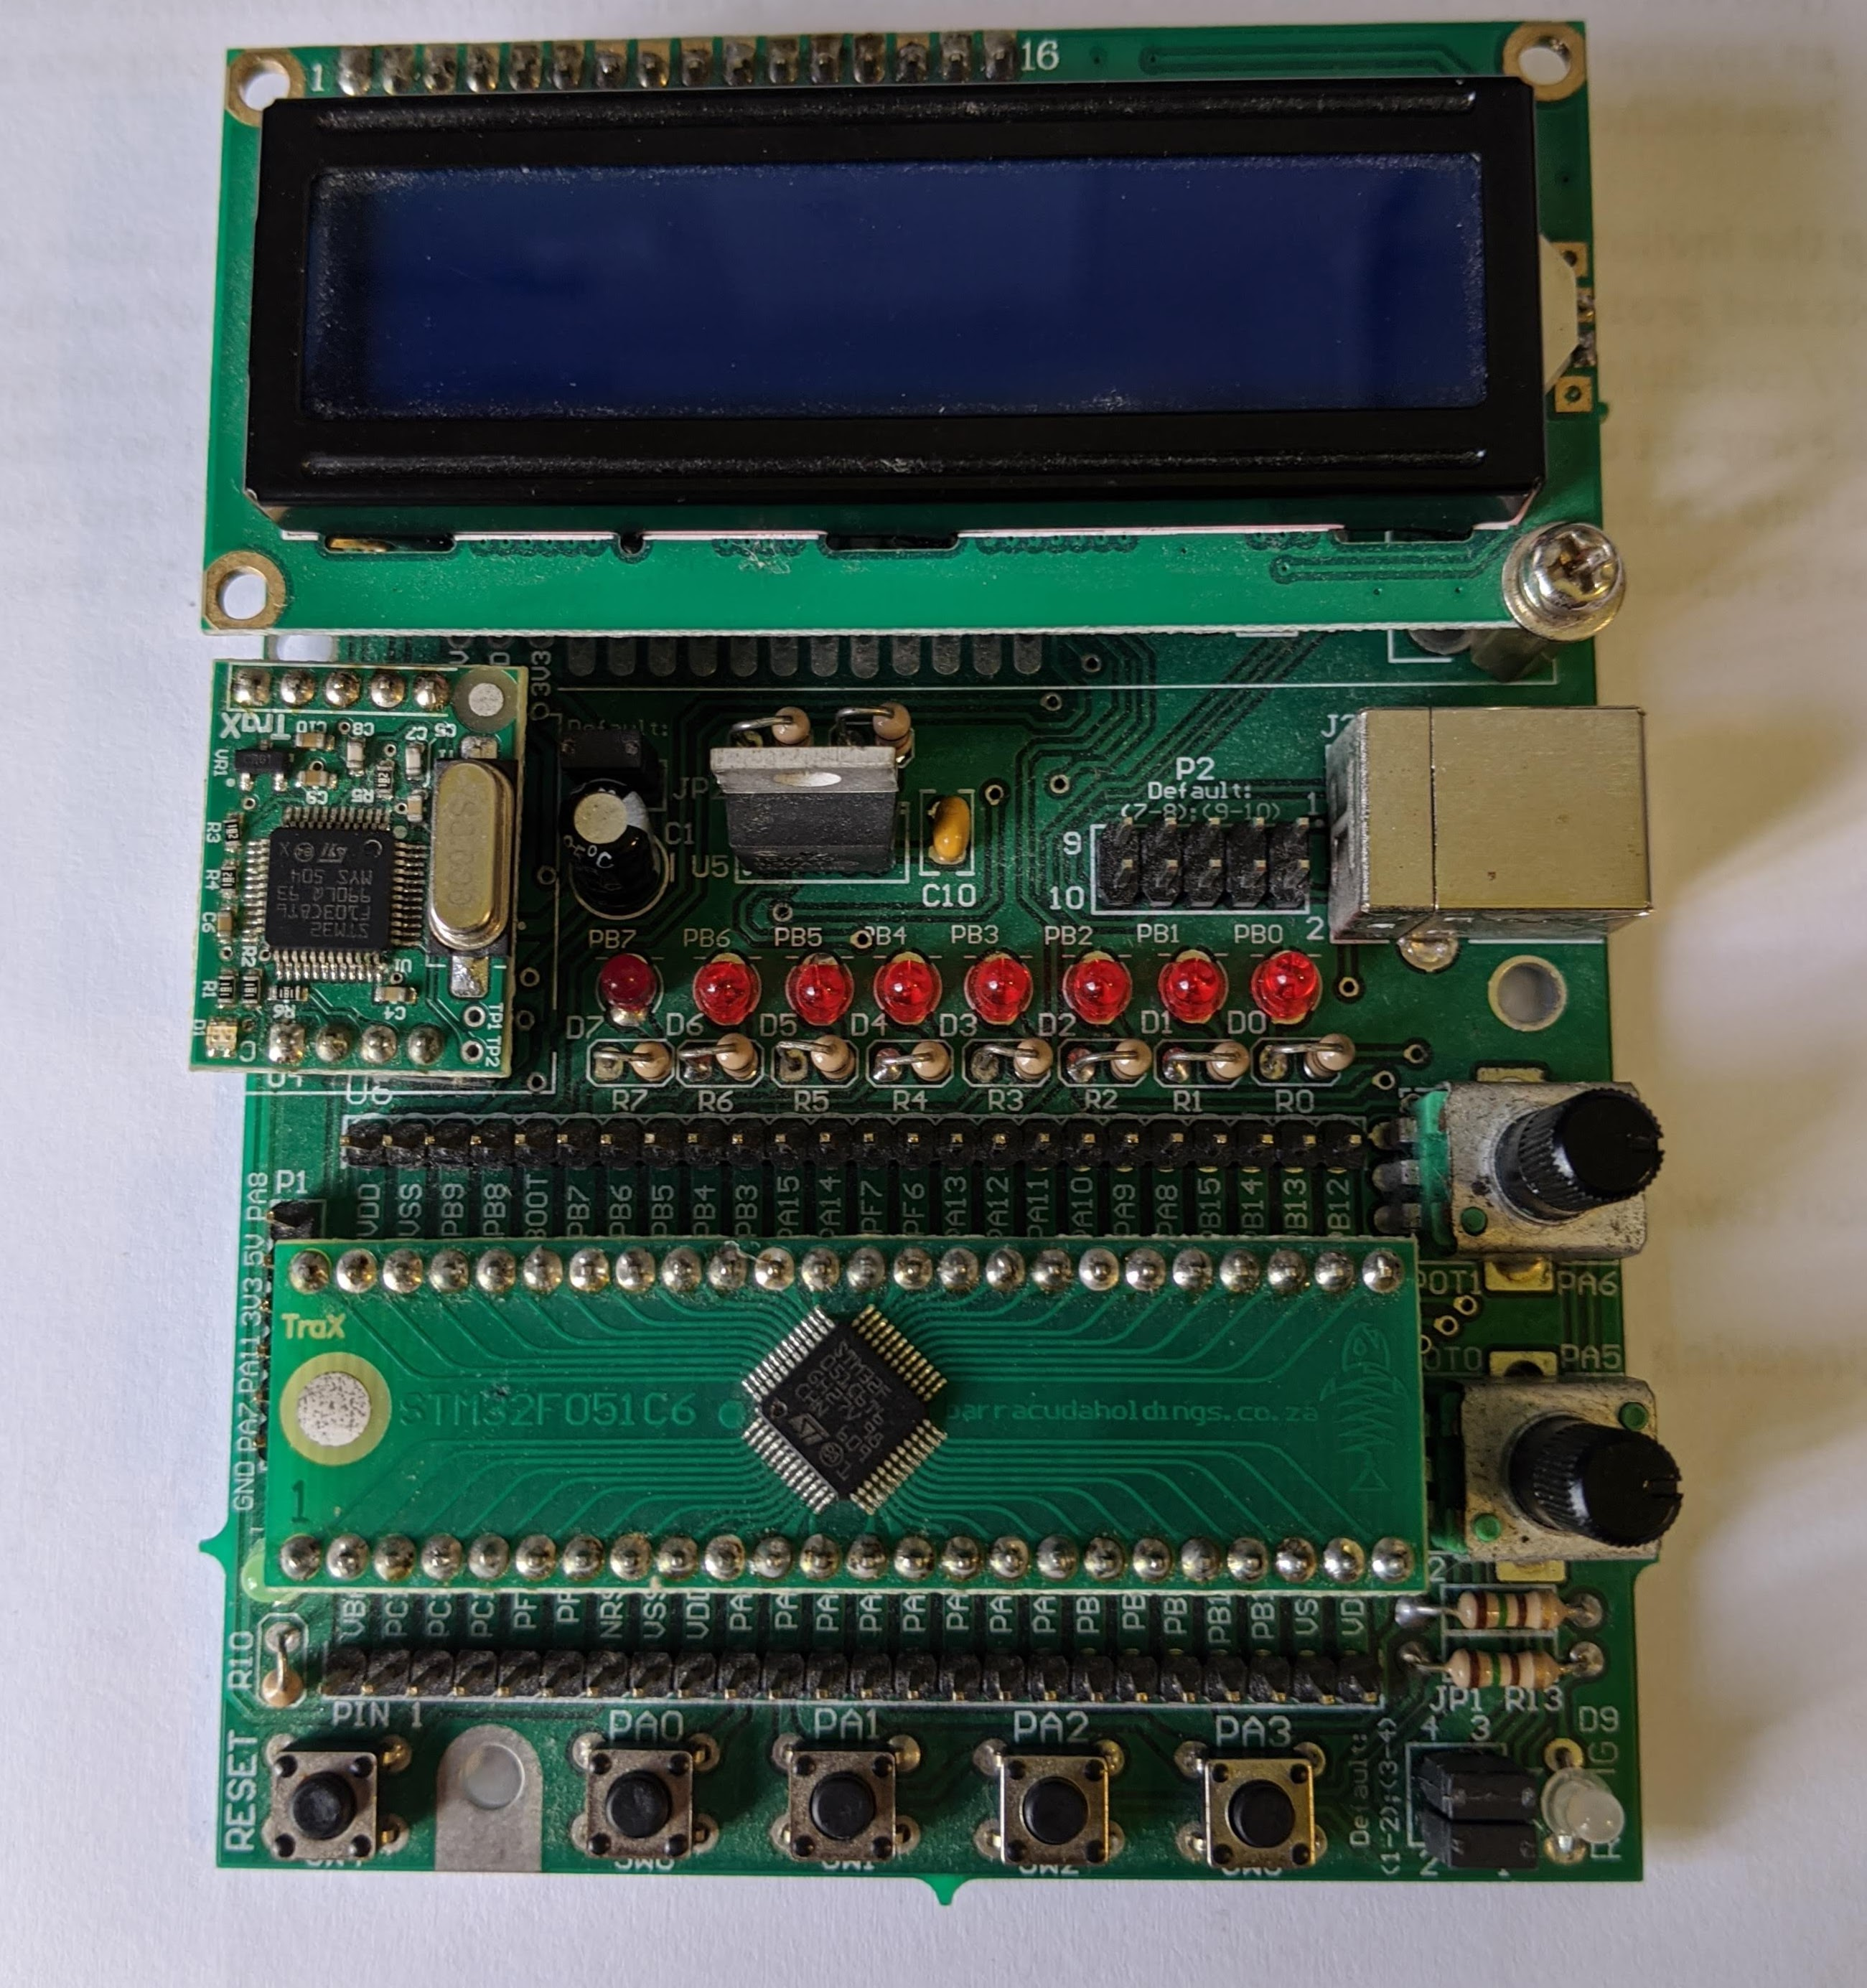
\includegraphics[width=.5\textwidth]{figures/design/dev_board_image.jpg}
	\caption{UCT STM32 Development Board}
	\label{fig:stm32_dev_board}
\end{figure}



%%%%%%%%%%%%%%%%%%%%%%%%%%%%%%%%%%%%%%%%%%%%%%%%%%%%%%%%%%%



\subsection{Carrier Frequency Generator}
\subsubsection{Functional Design}
To generate the 36kHz carrier waveform the LM555 timer IC was used. The module is designed to receive a 3.3V control signal. When a high logic level is received, the module switches the output at 36kHz to produce a square waveform.

The LED driver modules designed to be controlled by an open-collector, therefore a transistor was used to convert the push-pull output of the 555 timer to an open-collector output.

The 555 timer operates on 5V logic, transistors were used to convert the 3.3V control signal of the MCU to a 5V input on the RST pin of the 555 timer chip.

\subsubsection{Schematic}
Figure \ref{fig:schematic_carrier_generation} below shows the schematic for this module.

\begin{figure}[H]
	\centering
	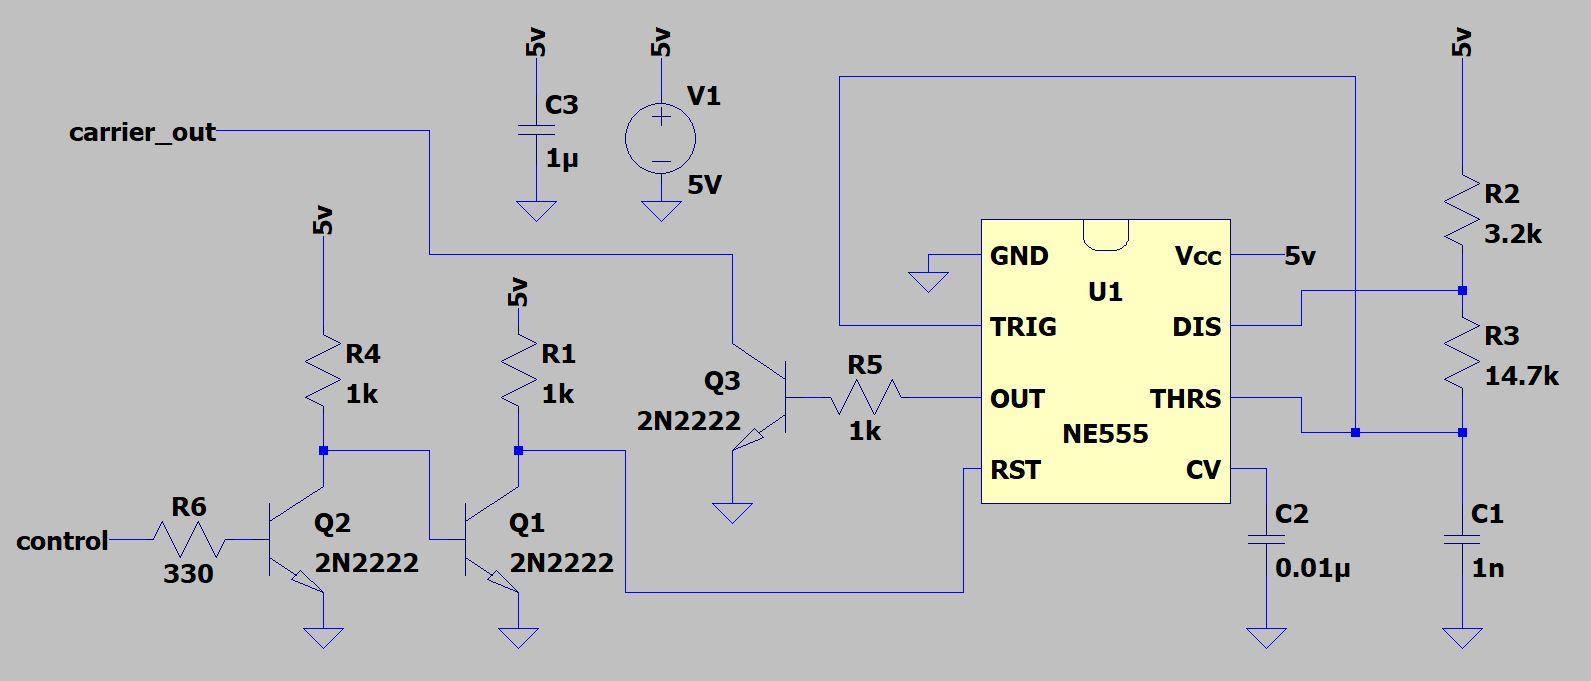
\includegraphics[width=.8\textwidth]{figures/design/carrier_waveform_generator_555.JPG}
	\caption{Carrier Generation Module Schematic}
	\label{fig:schematic_carrier_generation}
\end{figure}

\subsubsection{Frequency Generation}

According to the data sheet, the period of oscillation is governed by the following equation \(T = 0.693\times (R_2 + 2R_3)\times C_1\). The value of $C_1$ was chosen to be 1nF. To achieve the desired oscillation period of $27.7\mu S$, resistances $R_2$ and $R_3$ had to be chosen such that the relationship $(R_2 + 2R_3) = 40k\Omega$ held.

Due to a lack of access to resistor values, the circuit was implemented on a breadboard and resistors were combined to set $R_2$ and $R_3$, using the aforementioned relationship to guide the process. An oscilloscope was used to measure the output frequency and confirm the resulting frequency was suitable before implementing the design on strip-board.

The resistance values chosen were $R_2 = 3.2k\Omega$ and $R_3 = 14.7k\Omega$. According to the data sheet, these values produce an oscillation period of \(T_{theoretical} = 22.6\mu S\), however the actual period was measured to be \(T_{measured} = 26\mu S\) during burst operation.

The duty cycle is specified by the data sheet to be \(D_{theoretical} = \frac{R_3}{R_2\: +\: 2\times R_3}\), the expected duty cycle for this circuit design is 45\%.

\subsubsection{Module Realization}
The strip-board implementation of the module is shown in figure \ref{fig:module_carrier_generation} below.

\begin{figure}[H]
	\centering
	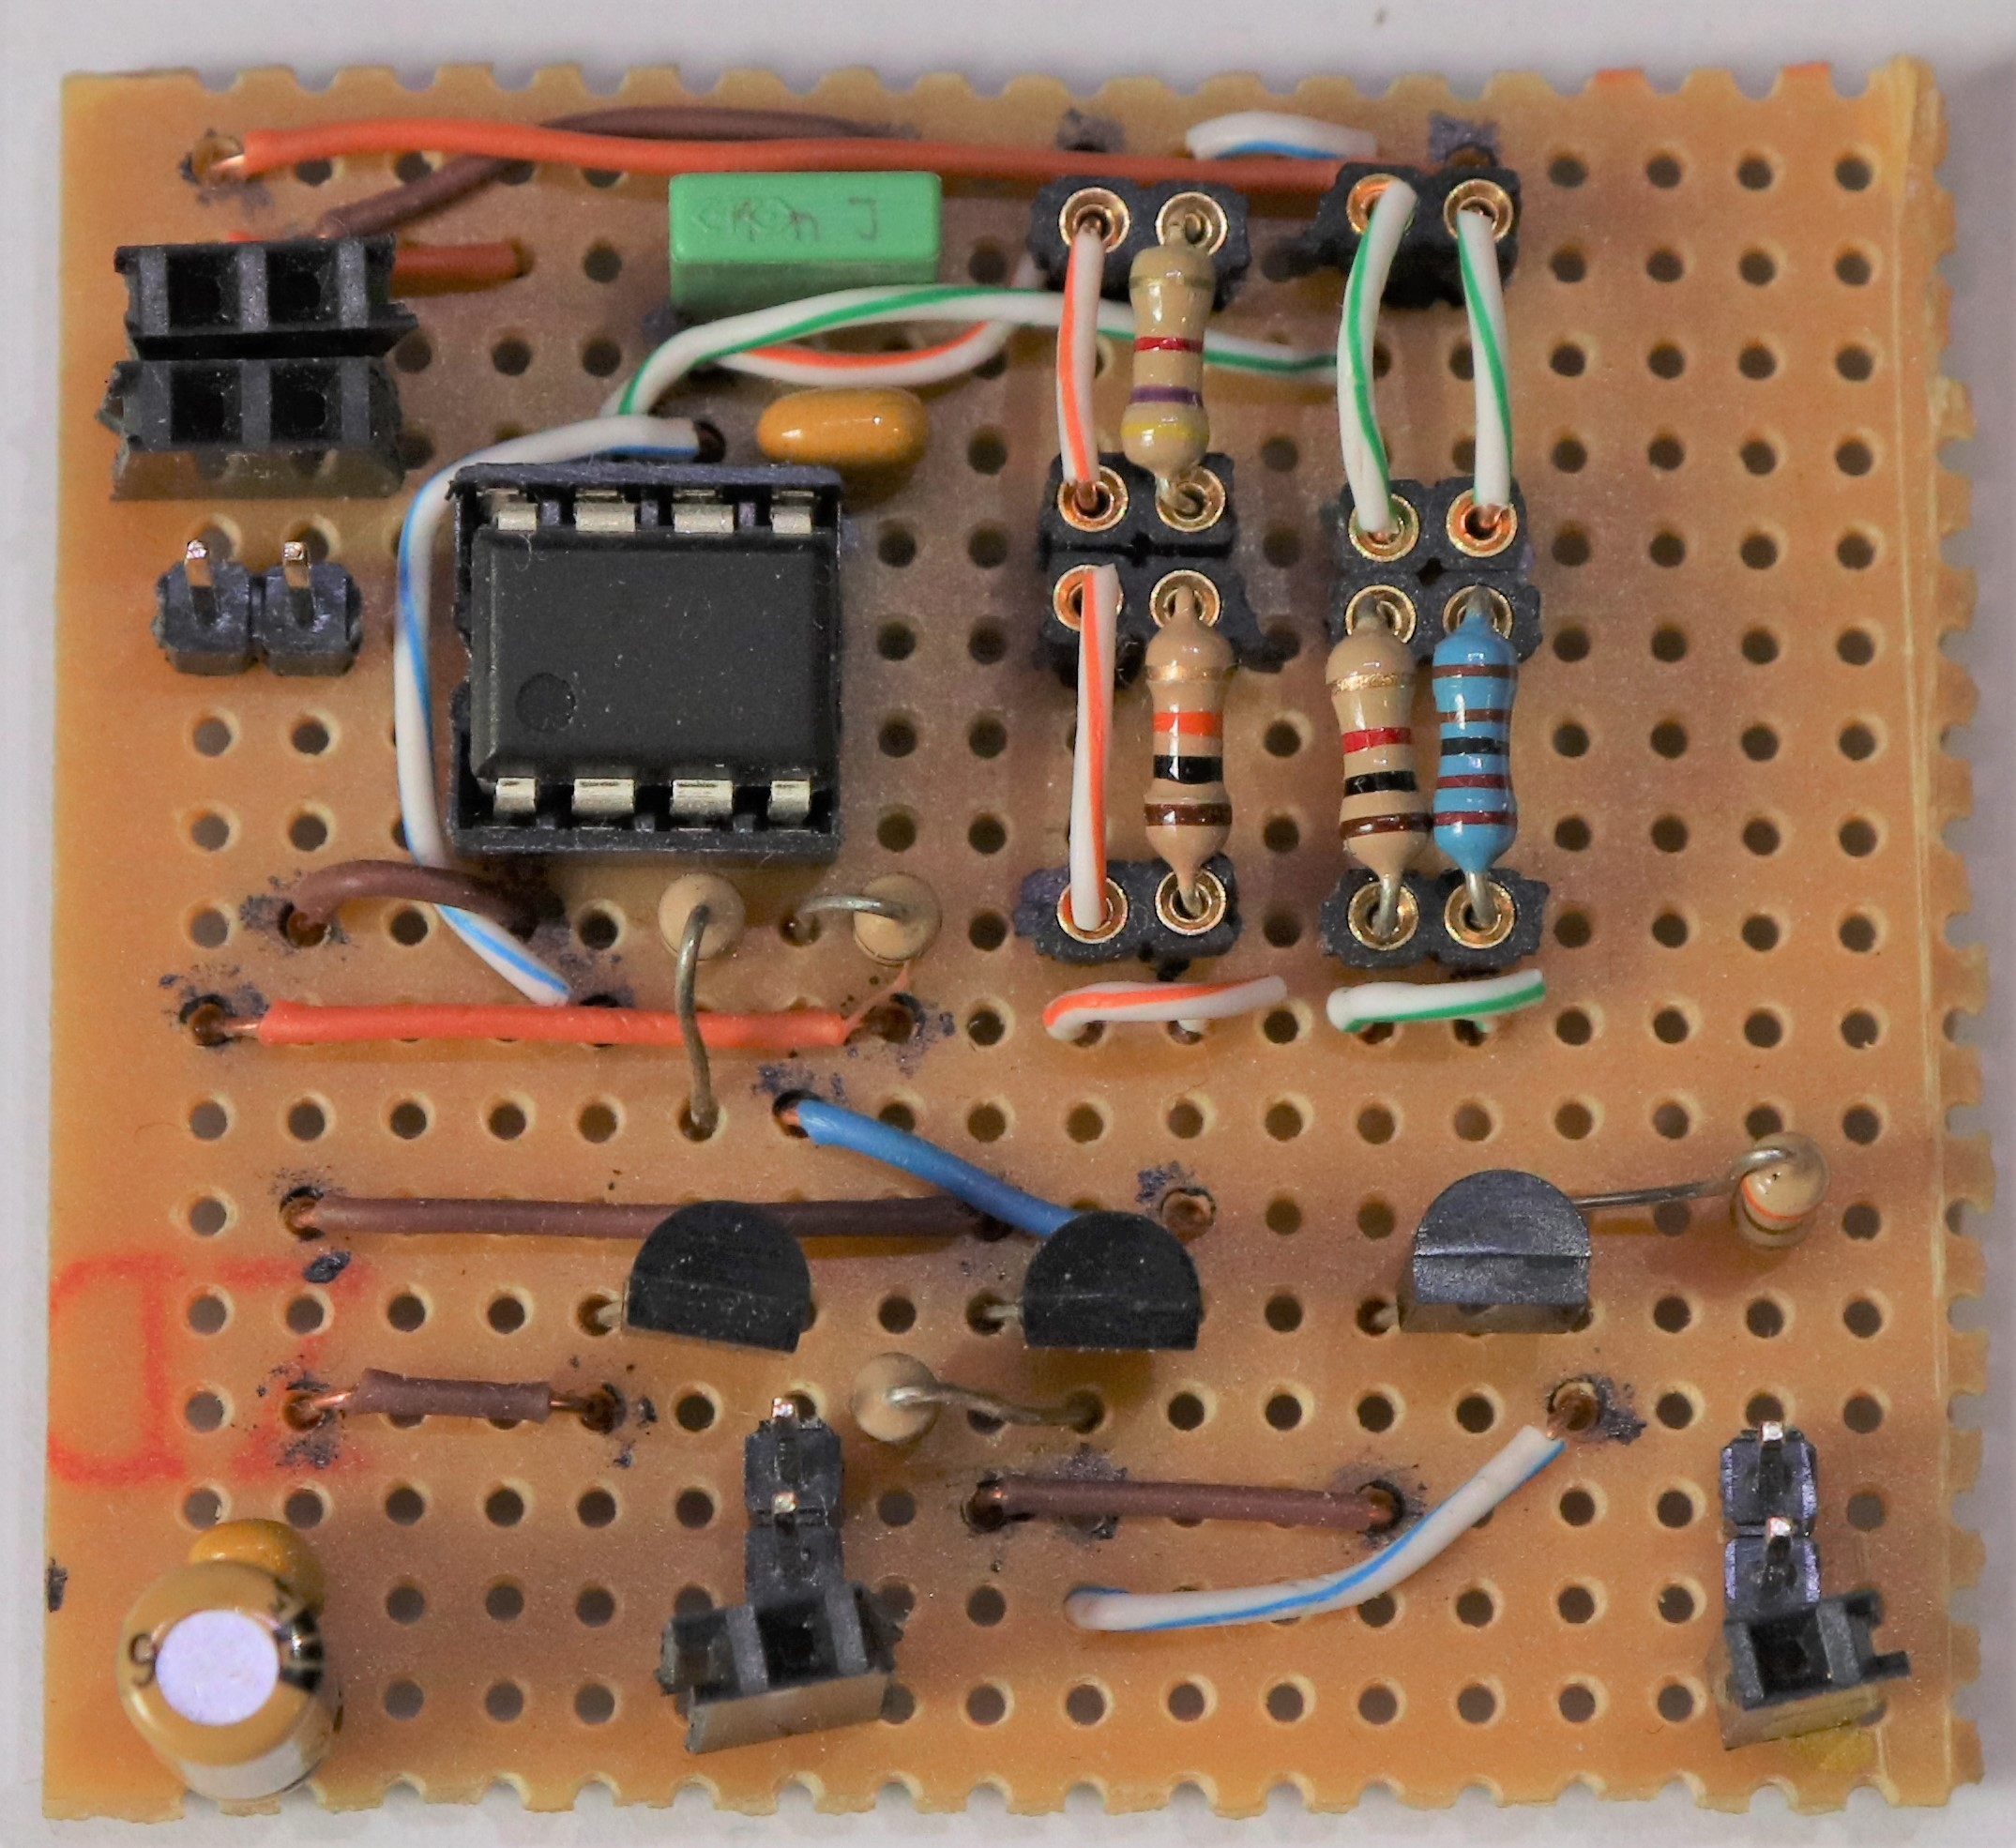
\includegraphics[width=.6\textwidth]{figures/modules/carrier_generator.jpg}
	\caption{Carrier Generation Module}
	\label{fig:module_carrier_generation}
\end{figure}



%%%%%%%%%%%%%%%%%%%%%%%%%%%%%%%%%%%%%%%%%%%%%%%%%%%%%%%%%%%



\subsection{Power LED Driver}

\subsubsection{Functional Design}
To operate the 3W high power IR LED a constant current driver must be implemented. The module is designed to be controlled by an open-collector control signal such that when the control signal is pulled low the led is illuminated. The output of this module is a constant current designed to drive a power LED.

The LED is to be modulated at 36kHz, typical LED drivers that utilize a switching regulator are not suitable for regulating the current at such high modulation frequencies. This is because the switching frequency used in commonly available constant current switching regulators is not high enough. Instead, a linear regulator was designed using discrete components.

\subsubsection{Schematic}
Figure \ref{fig:schematic_power_led_driver} shows the design of a high power linear regulator, built around the IRLZ44 enhancement PMOSFET. Heat-sinks were attached to both the high power LED and the IRLZ44 power MOSFET.

\begin{figure}[H]
	\centering
	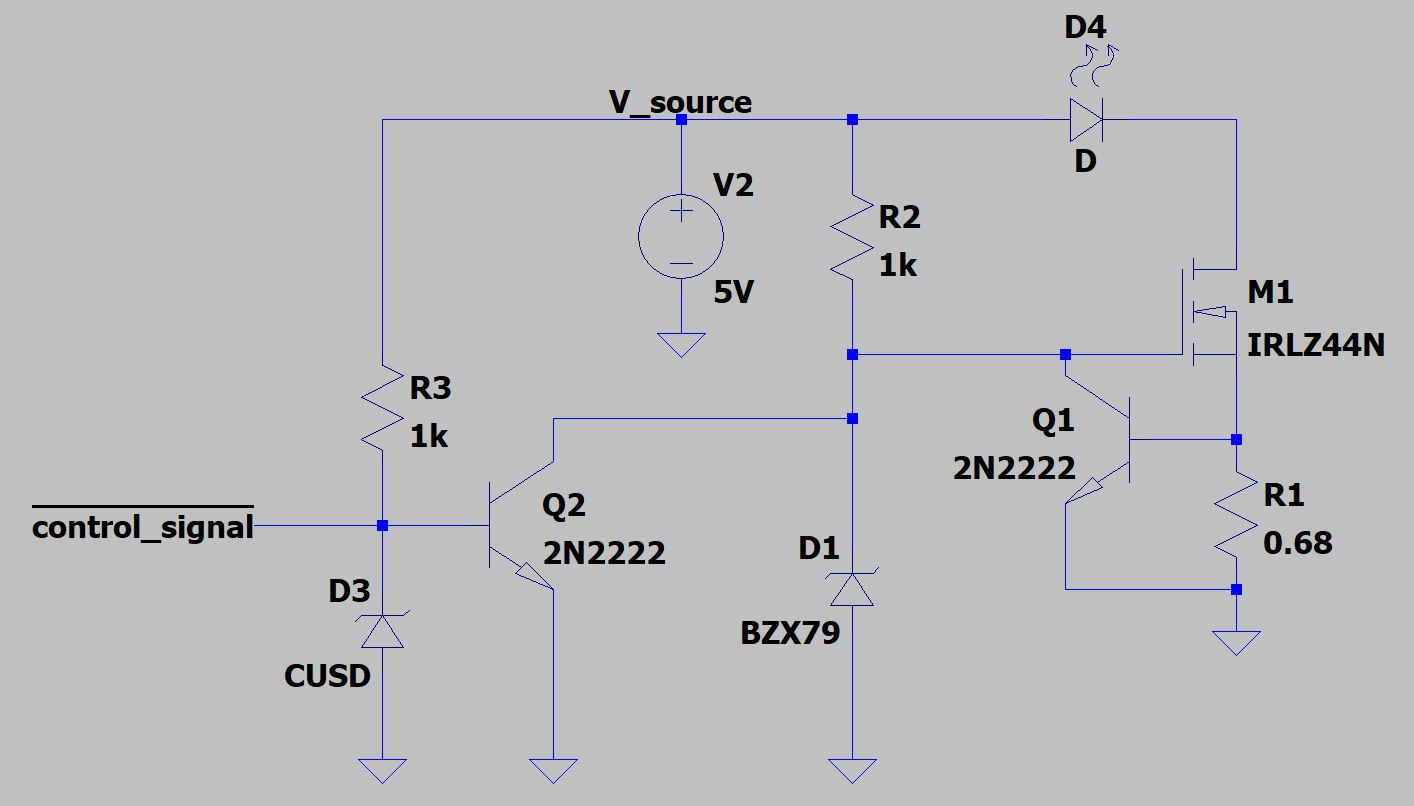
\includegraphics[width=.8\textwidth]{figures/design/power_led_driver.JPG}
	\caption{Power LED Driver Module Schematic}
	\label{fig:schematic_power_led_driver}
\end{figure}

\subsubsection{Constant Current Control}

Current regulation is performed by MOSFET M1, transistor Q1 and shunt resistor R1. When a sufficiently small current is flowing, the voltage drop across the R1 is negligible, so no current is allowed to flow from collector to emitter of Q1. Under these circumstances the gate of M1 is pulled high by R2 and current is allowed to flow through the LED.

As the current through R1 increases, the voltage across the base-emitter of Q1 overcomes the forward voltage and the transistor begins to conduct. This conduction pulls the gate of M1 to ground reducing the current flowing through the LED.

The maximum current ($I_{max}$) is set by choosing R1 such that the voltage across R1 is equal to the diode drop of the base-emitter of Q1. A conservative estimate for the diode drop is 0.7V.

R1 was chosen to be $0.68\Omega$, to achieve a current limit of just over 1A.


\subsubsection{Module Realization}
The strip-board implementation of the module is shown in figure \ref{fig:module_power_led_driver} below.

\begin{figure}[H]
	\centering
	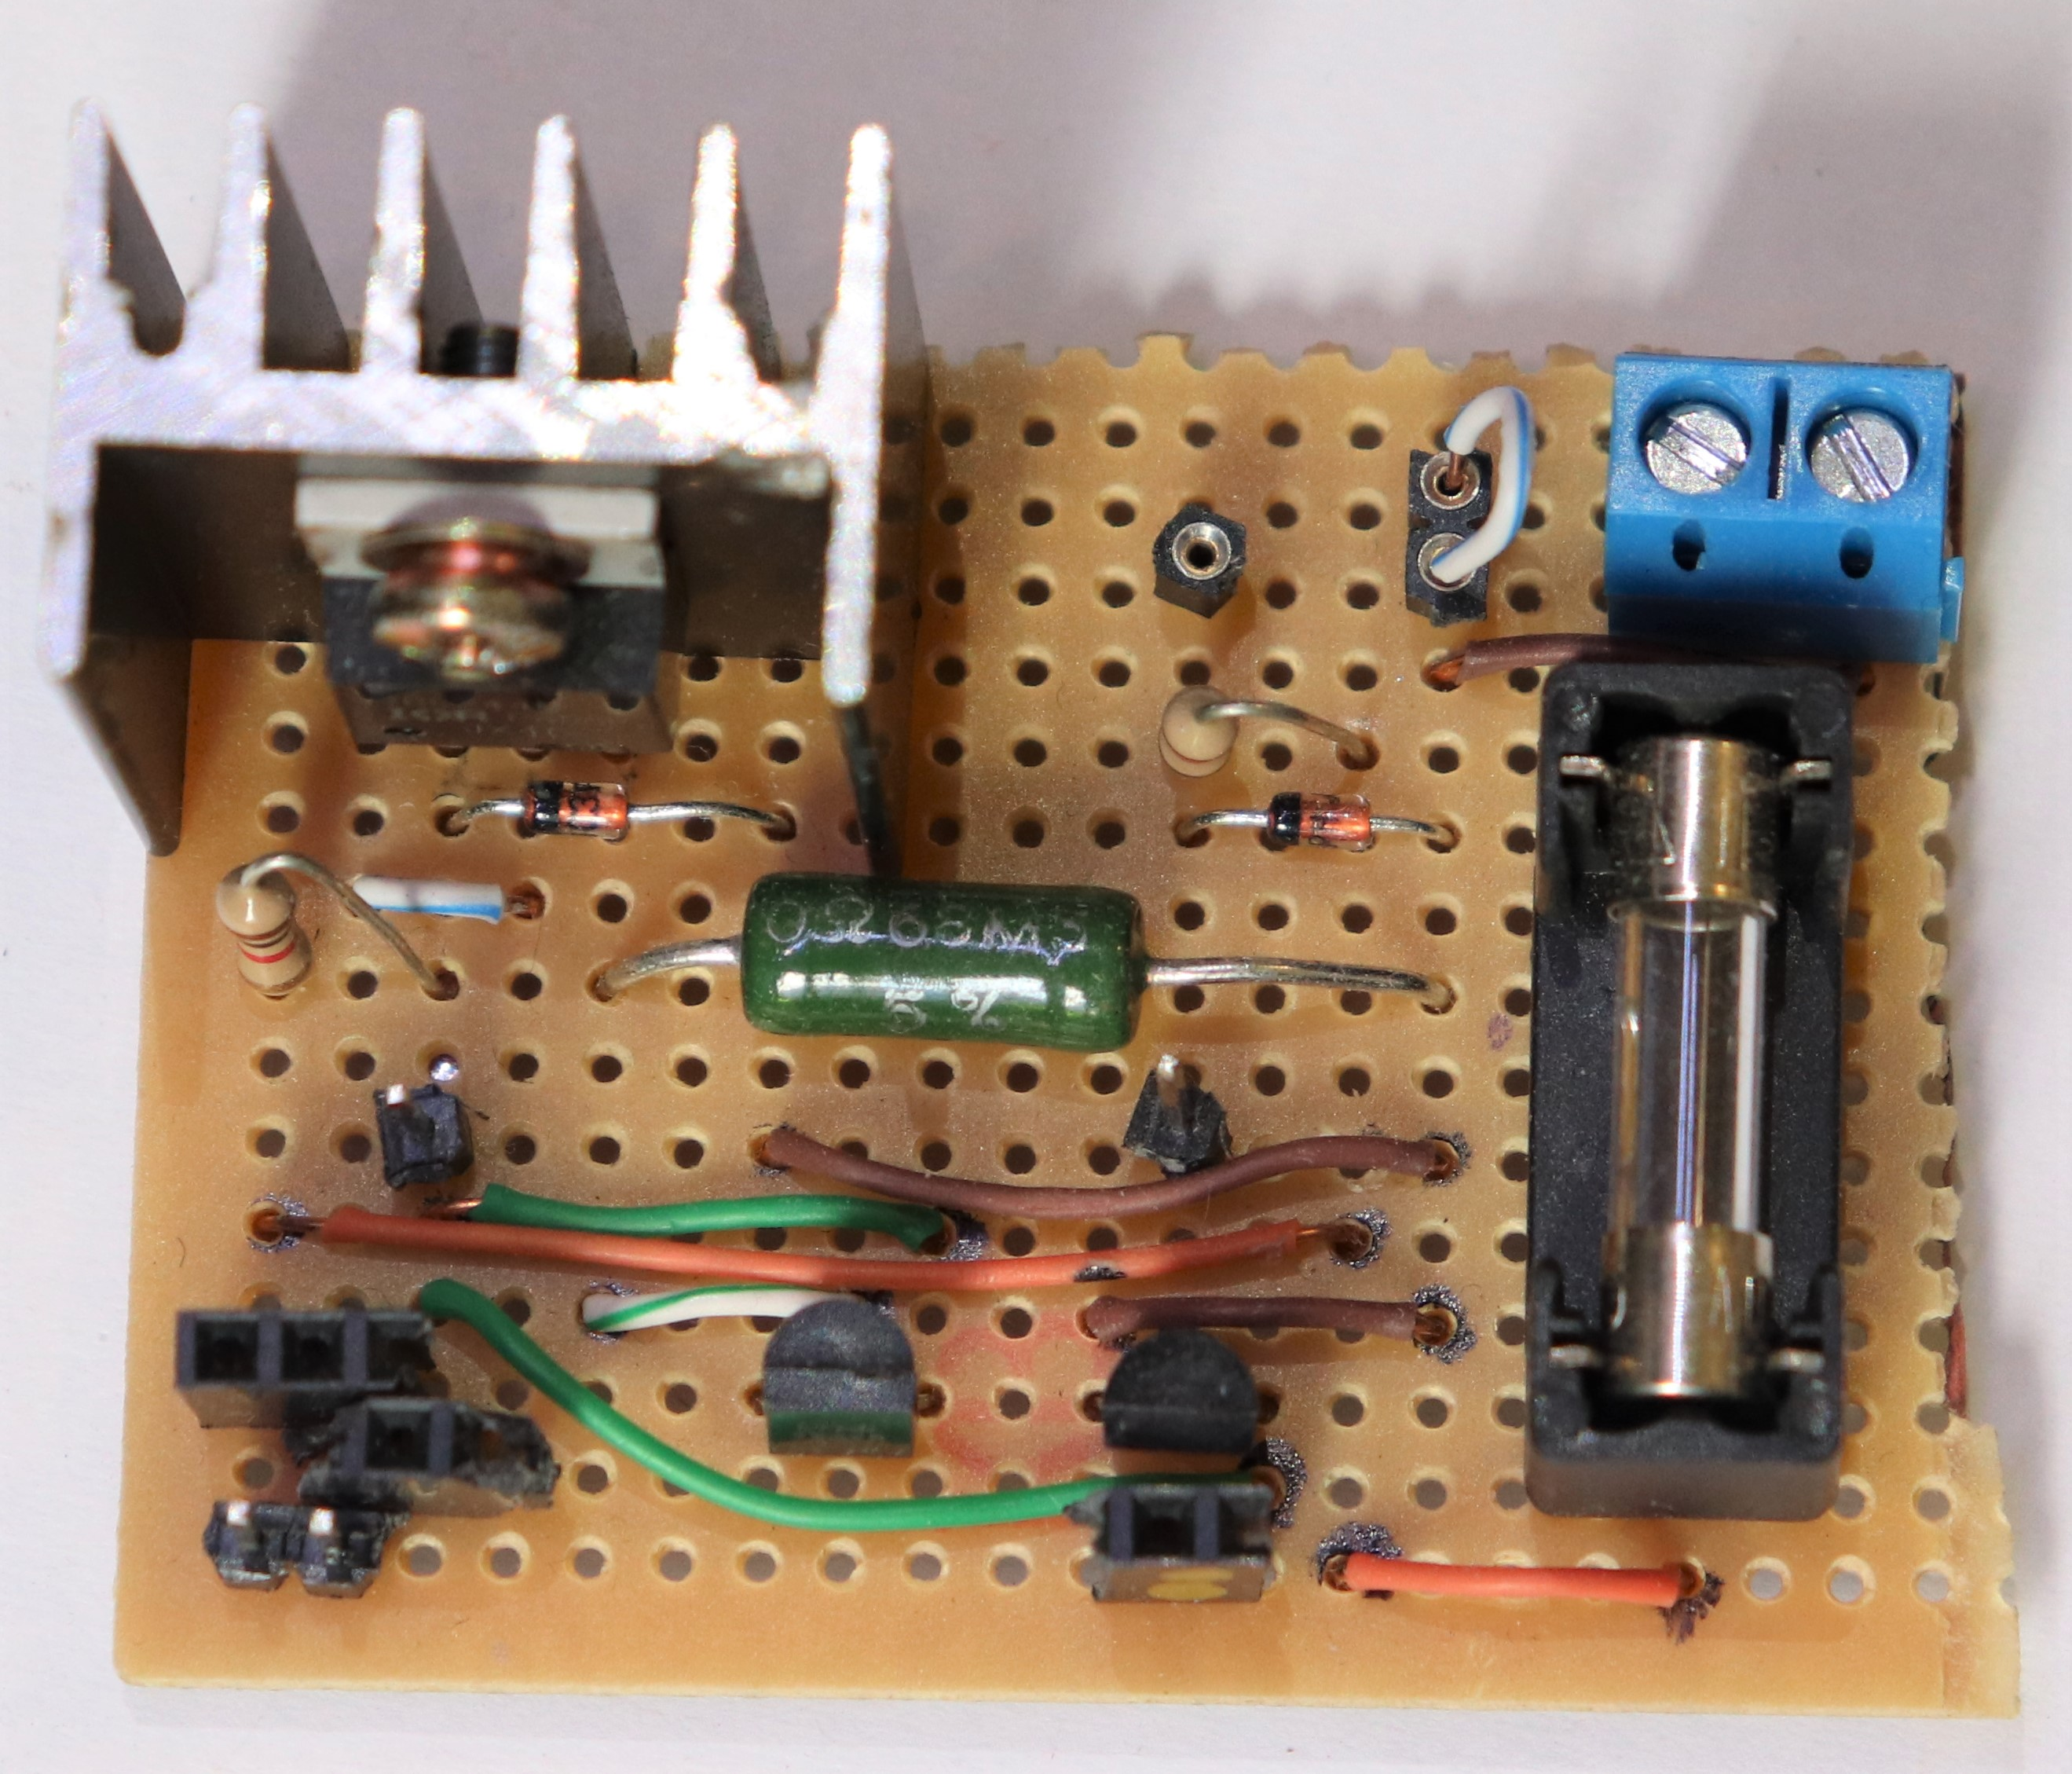
\includegraphics[width=.6\textwidth]{figures/modules/power_led_driver.jpg}
	\caption{Power LED Driver Module}
	\label{fig:module_power_led_driver}
\end{figure}



%%%%%%%%%%%%%%%%%%%%%%%%%%%%%%%%%%%%%%%%%%%%%%%%%%%%%%%%%%%




\subsection{LED Driver}

\subsubsection{Functional Design}
Due to the high power demands of the 3W IR LED, it is more appropriate to use a low power IR led during the development of the communication protocol. A separate low power LED driver module was designed for this specific purpose.

The module is designed to be pin-to-pin compatible with the power LED driver module, operating on the same input signal produced by an open-collector driven pin. Pulling the input low causes the LED to illuminate.



\subsubsection{Schematic}
Figure \ref{fig:schematic_low_power_led_driver} shows the schematic for this driver module.

\begin{figure}[H]
	\centering
	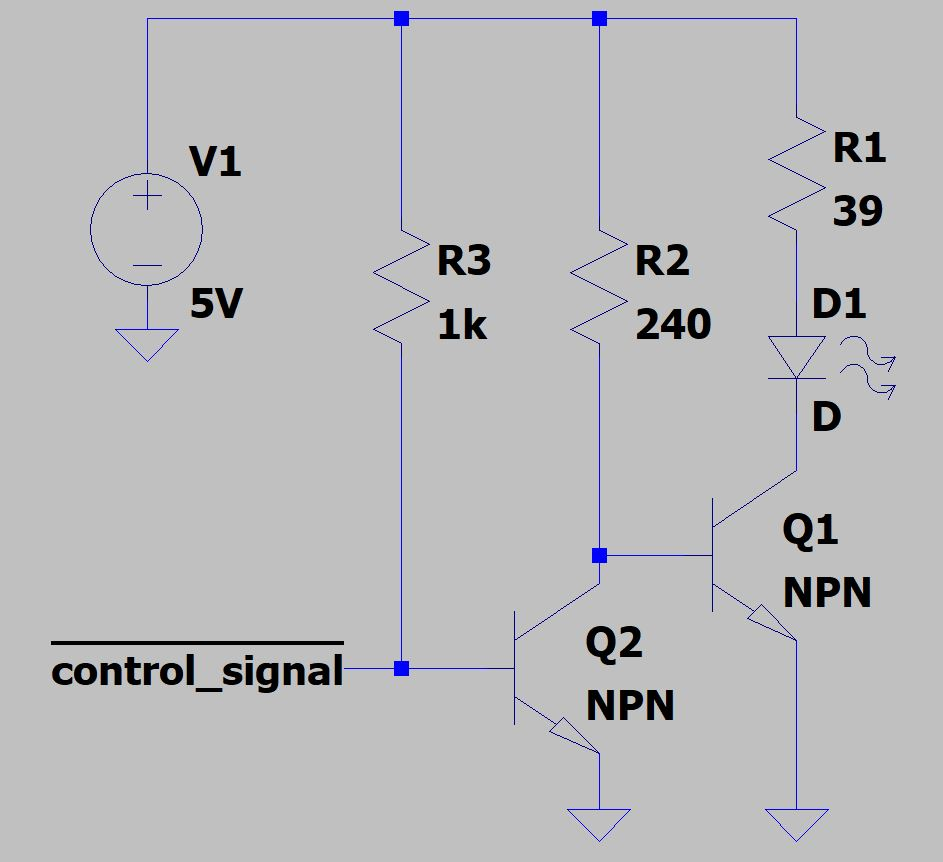
\includegraphics[width=.6\textwidth]{figures/design/low_power_led_driver.JPG}
	\caption{Low-Power LED Driver Module Schematic}
	\label{fig:schematic_low_power_led_driver}
\end{figure}

A $39\Omega$ resistor is used to regulate the current through the LED. The pair of NPN transistors are used to switch the LED per the signal generated by an open-collector control signal.

\subsubsection{Module Realization}
The strip-board implementation of the module is shown in figure \ref{fig:module_led_driver} below.

\begin{figure}[H]
	\centering
	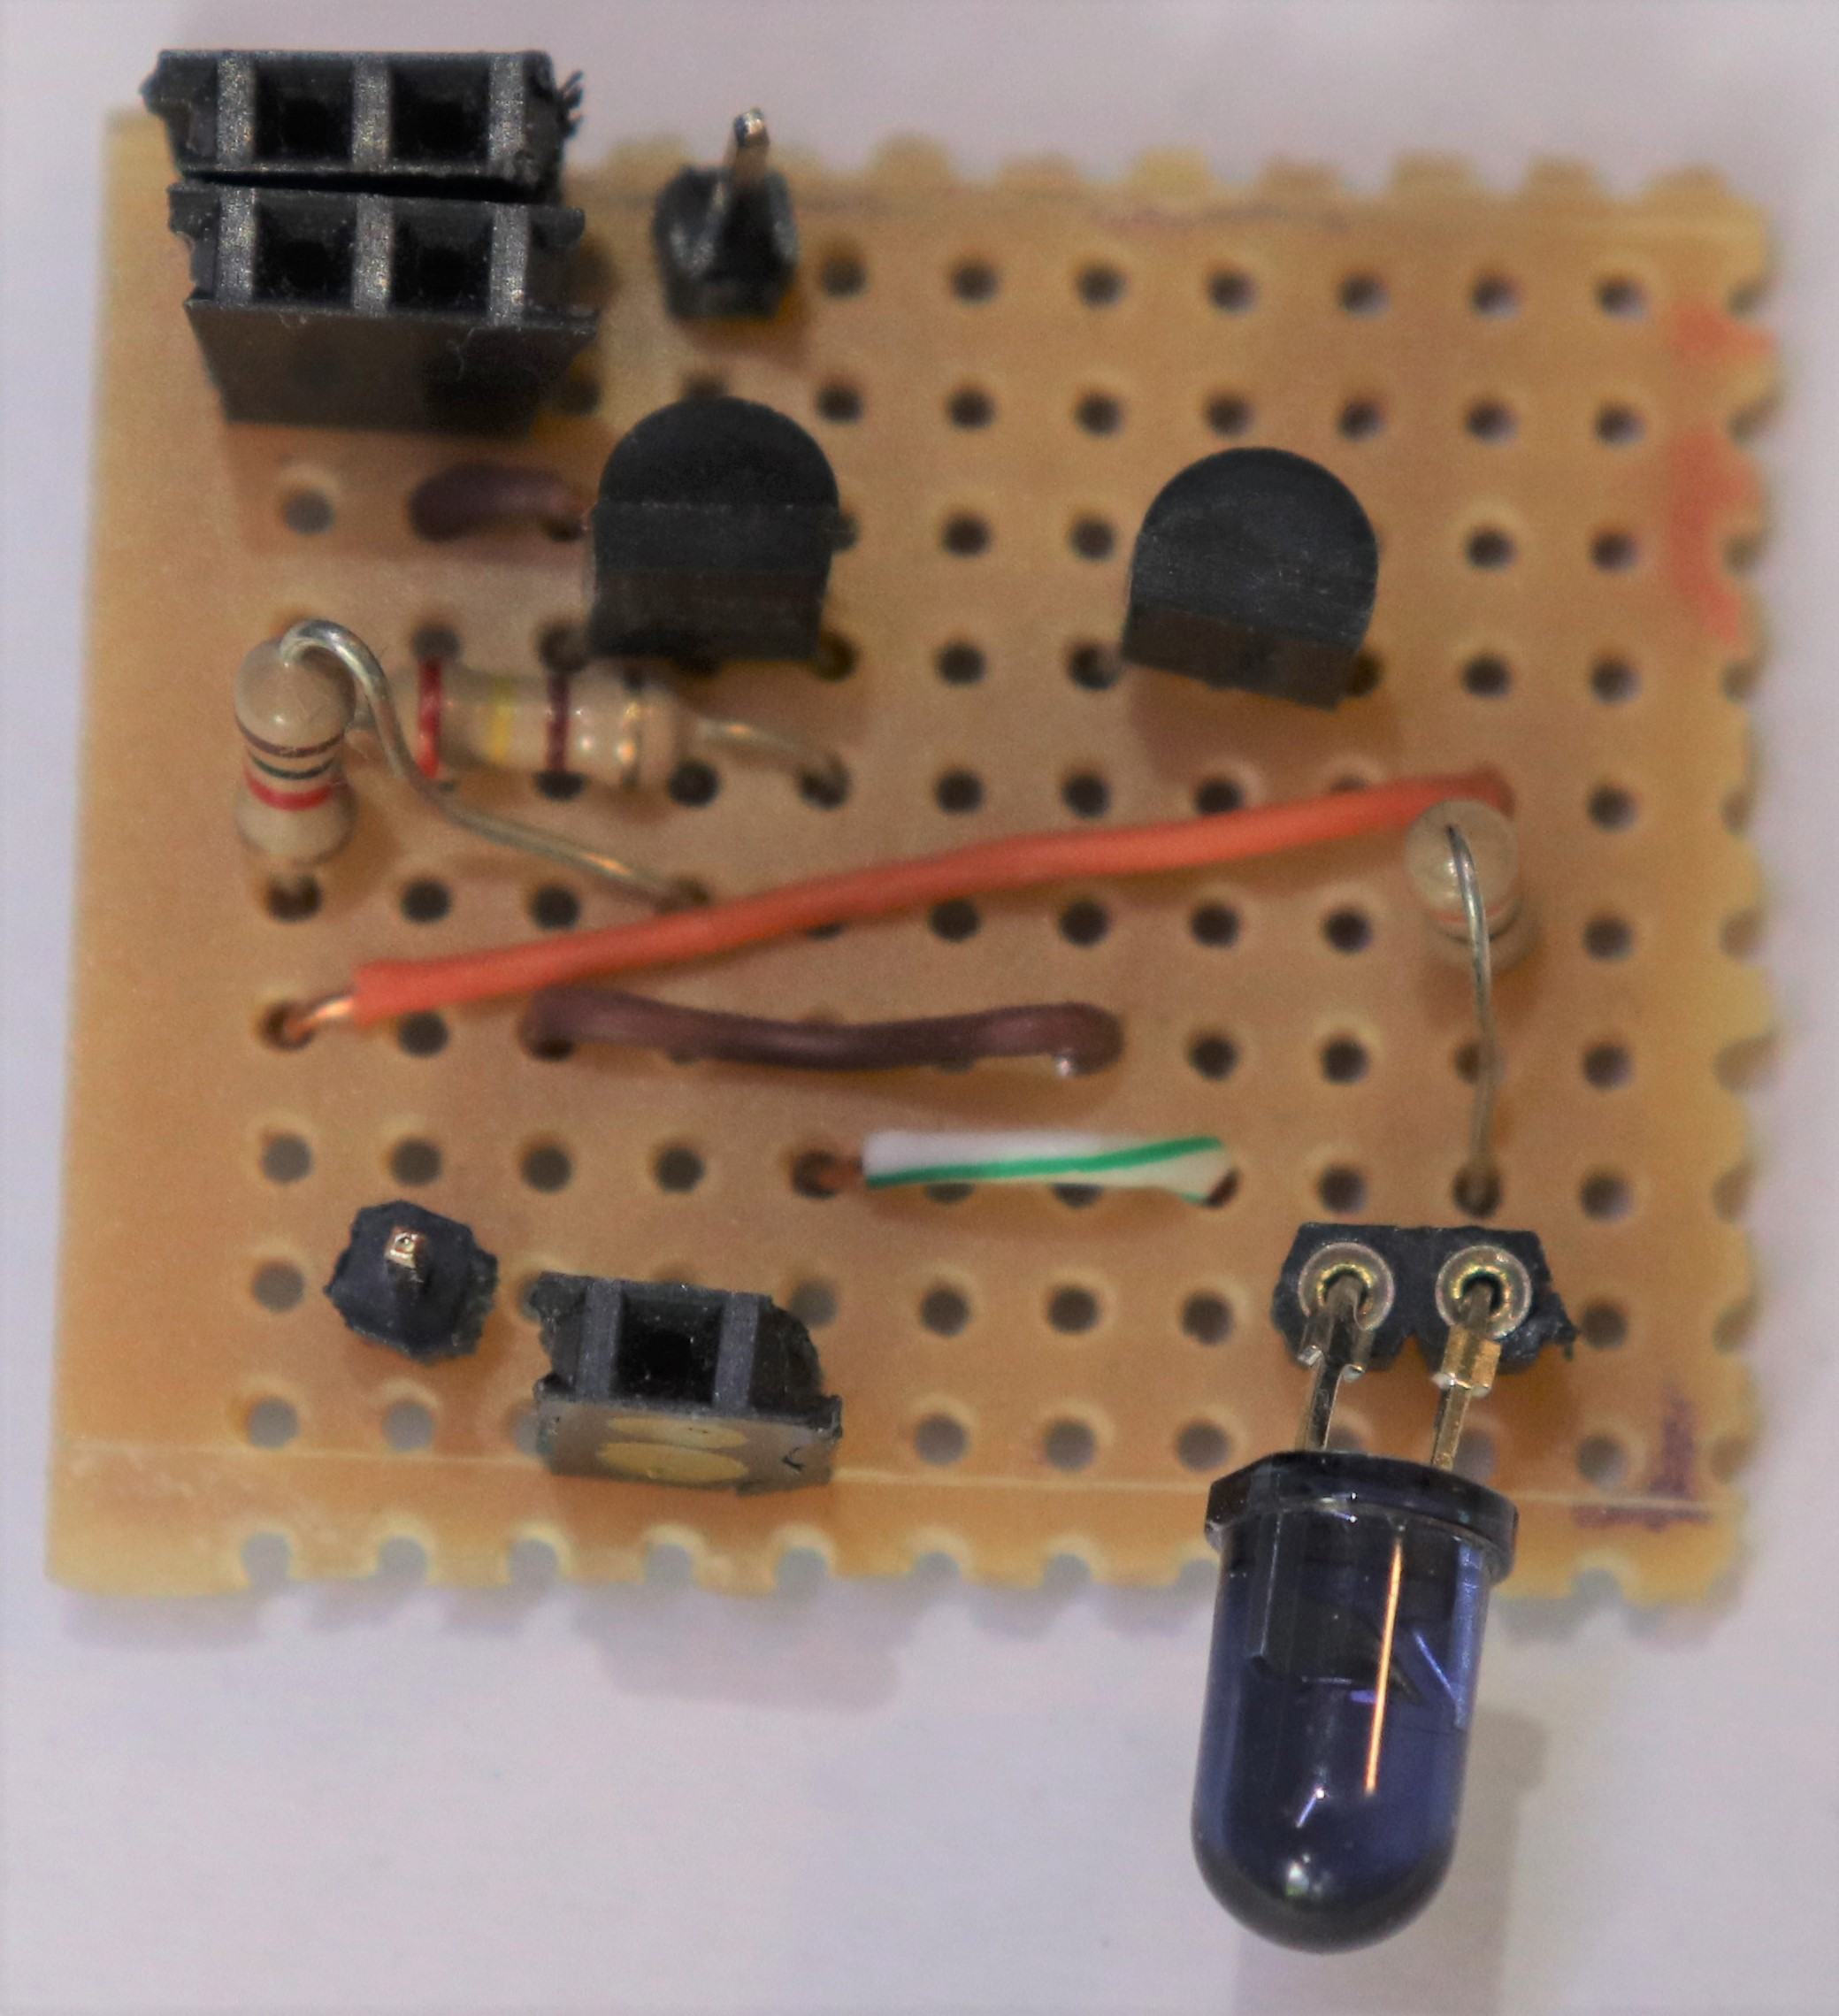
\includegraphics[width=.6\textwidth]{figures/modules/led_driver.jpg}
	\caption{LED Driver Module}
	\label{fig:module_led_driver}
\end{figure}




%%%%%%%%%%%%%%%%%%%%%%%%%%%%%%%%%%%%%%%%%%%%%%%%%%%%%%%%%%%




\subsection{Light Focus System}

\subsubsection{Functional Design}
The high power IR LED has a nominally wide beam angle. The function of the light focus system is to efficiently generate a narrow beam of IR from this light source. This was achieved by using a lens to focus the light into a parallel beam and using a tube to prevent the light not passing through the lens from spilling into the surrounding environment.


\subsubsection{Construction}
Figure \ref{fig:light_focusing_tube} below shows an exploded view of this hardware module. The diagram lists the components used to construct the light focusing tube.

\begin{figure}[H]
	\centering
	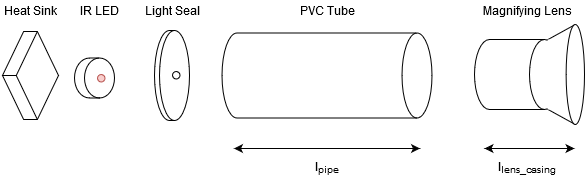
\includegraphics[width=.8\textwidth]{figures/design/beam_tube.png}
	\caption{Exploded View - Light Focusing Tube}
	\label{fig:light_focusing_tube}
\end{figure}

\paragraph{Component Dimensions}
The magnifying lens casing had a length of 30mm, the lens is in-set by 1mm and 3mm of the casing remains external to the tube. The experimental result from section \ref{exp:focal_length} calculated the focal length to be 53mm. The lens itself has a diameter of 22mm.

\subsubsection{Light Focusing}

A narrow beam of parallel rays of light may be formed using a point source and ideal lens. Approximating the LED as a point source and the magnifying lens as ideal, a narrow beam may be generated by positioning the light source one focal length away from the lens.

The distance between the light source and lens can be calculated according to equation \ref{eqn:tube_length}.

\begin{equation}
d_{source-lens} = l_{tube} - l_{lens\_casing} + (l_{lens\_inset\_distance} + l_{lens\_external}) + l_{light\_seal\_thickness}
\label{eqn:tube_length}
\end{equation}

$d_{source-lens}$ is the distance between the light source and the lens. $l_{tube}$ is the length of the tube. $l_{lens\_casing}$ is the length of the magnifying lens casing as illustrated in figure \ref{fig:light_focusing_tube}, $l_{lens\_inset\_distance}$ is the amount by which the lens is in-set inside the casing and $l_{lens\_external}$ is a measure of the length of casing that remains external to the tube. $l_{light\_seal\_thickness}$ is a measure of the thickness of the hard-board used to form the light seal.

The length $l_{tube}$ was calculated by substituting the experimentally determined focal length into the equation as the length $d_{source-lens}$.

Substituting these values into equation \ref{eqn:tube_length}, the length $l_{tube}$ was calculated

\[l_{tube} = d_{source-lens} + l_{lens\_casing} - (l_{lens\_inset\_distance} + l_{lens\_external}) - l_{light\_seal\_thickness}\]

\[l_{tube} = 53mm + 30mm - (1mm + 3mm) - 3mm = 76mm\]


\subsubsection{Module Realization}
The implementation of the light focus system is shown in figure \ref{fig:module_light_focus} below. Excluded from this image is the IR led and heat-sink.

\begin{figure}[H]
	\centering
	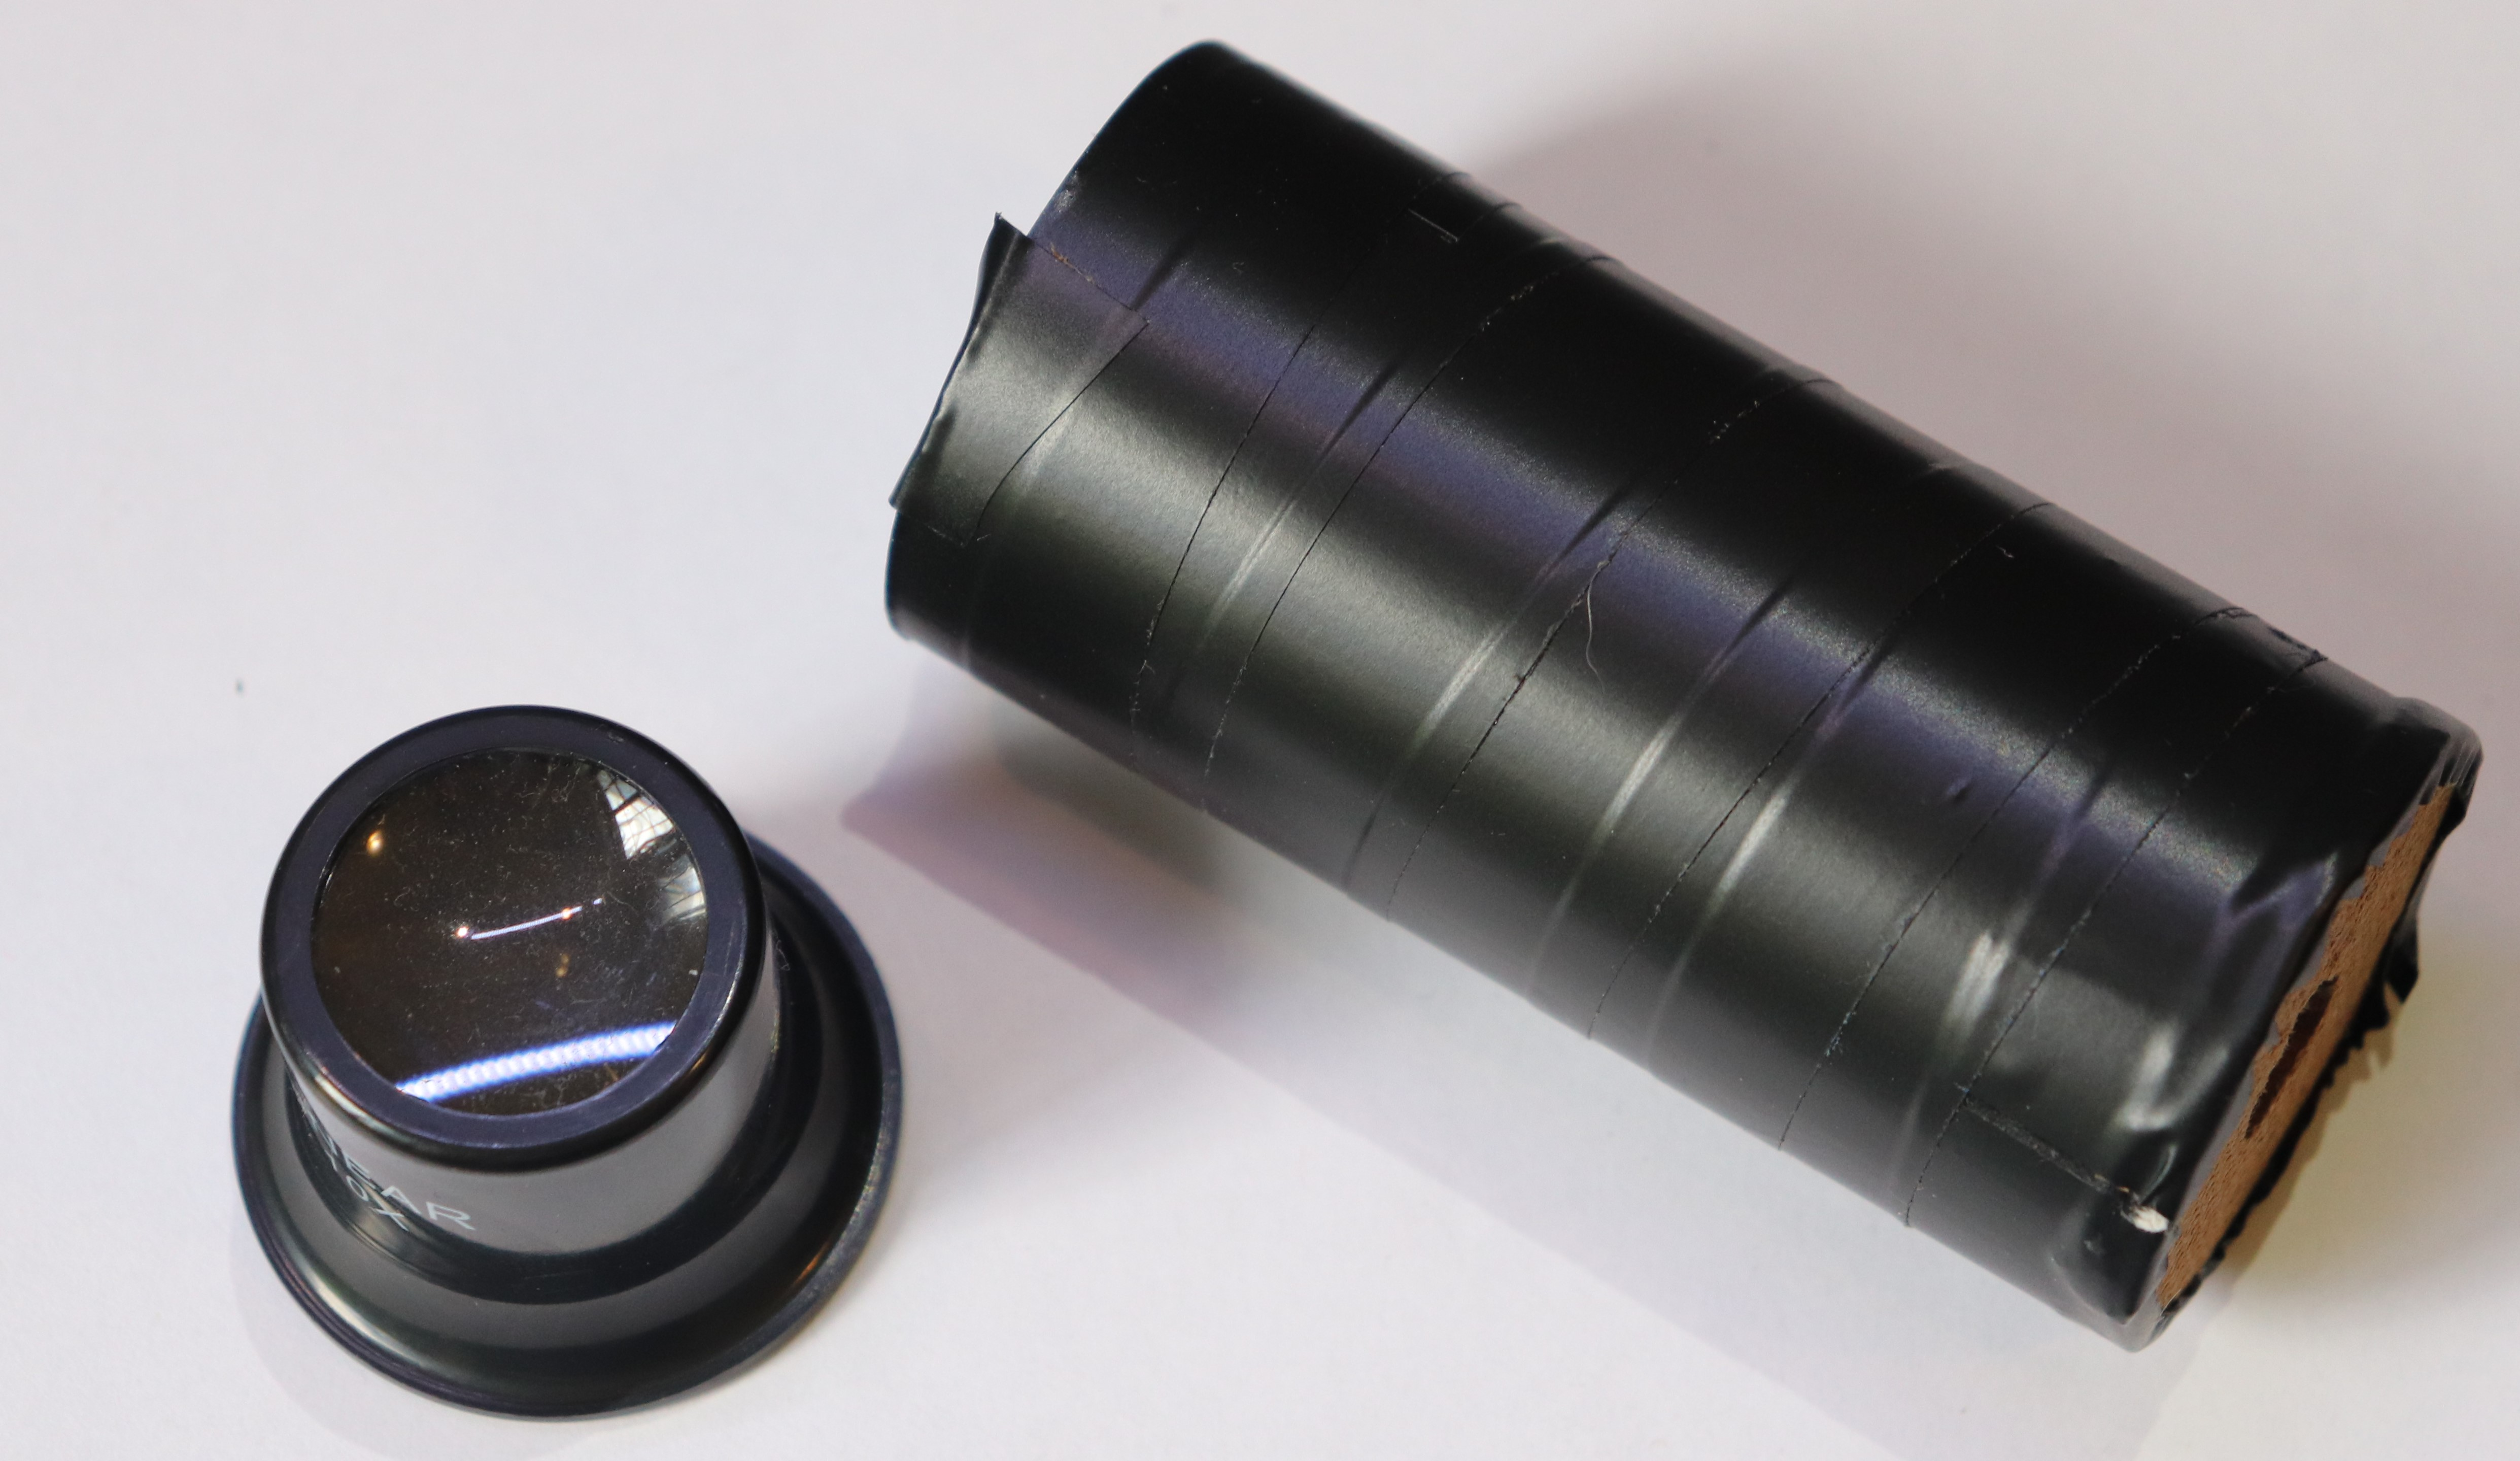
\includegraphics[width=.6\textwidth]{figures/modules/light_focus_tube_lens.jpg}
	\caption{Light Focus System}
	\label{fig:module_light_focus}
\end{figure}



%%%%%%%%%%%%%%%%%%%%%%%%%%%%%%%%%%%%%%%%%%%%%%%%%%%%%%%%%%%




\subsection{Photodiode IR Detector}

\subsubsection{Functional Design}
The photodiode IR detector module is designed to convert fluctuations in infrared radiation into a voltage signal. The circuit is designed to produce an output voltage proportional to changes in the current flowing through the photodiode.


\subsubsection{Schematic}
Figure \ref{fig:schematic_photodiode_transimpedance} below shows the schematic for this module. The circuit is an adaption of S. Schrires 'Infrared Radio Link' receiver circuit which may be found in the EEE3071 course notes \cite{Schrire2007}.

\begin{figure}[H]
	\centering
	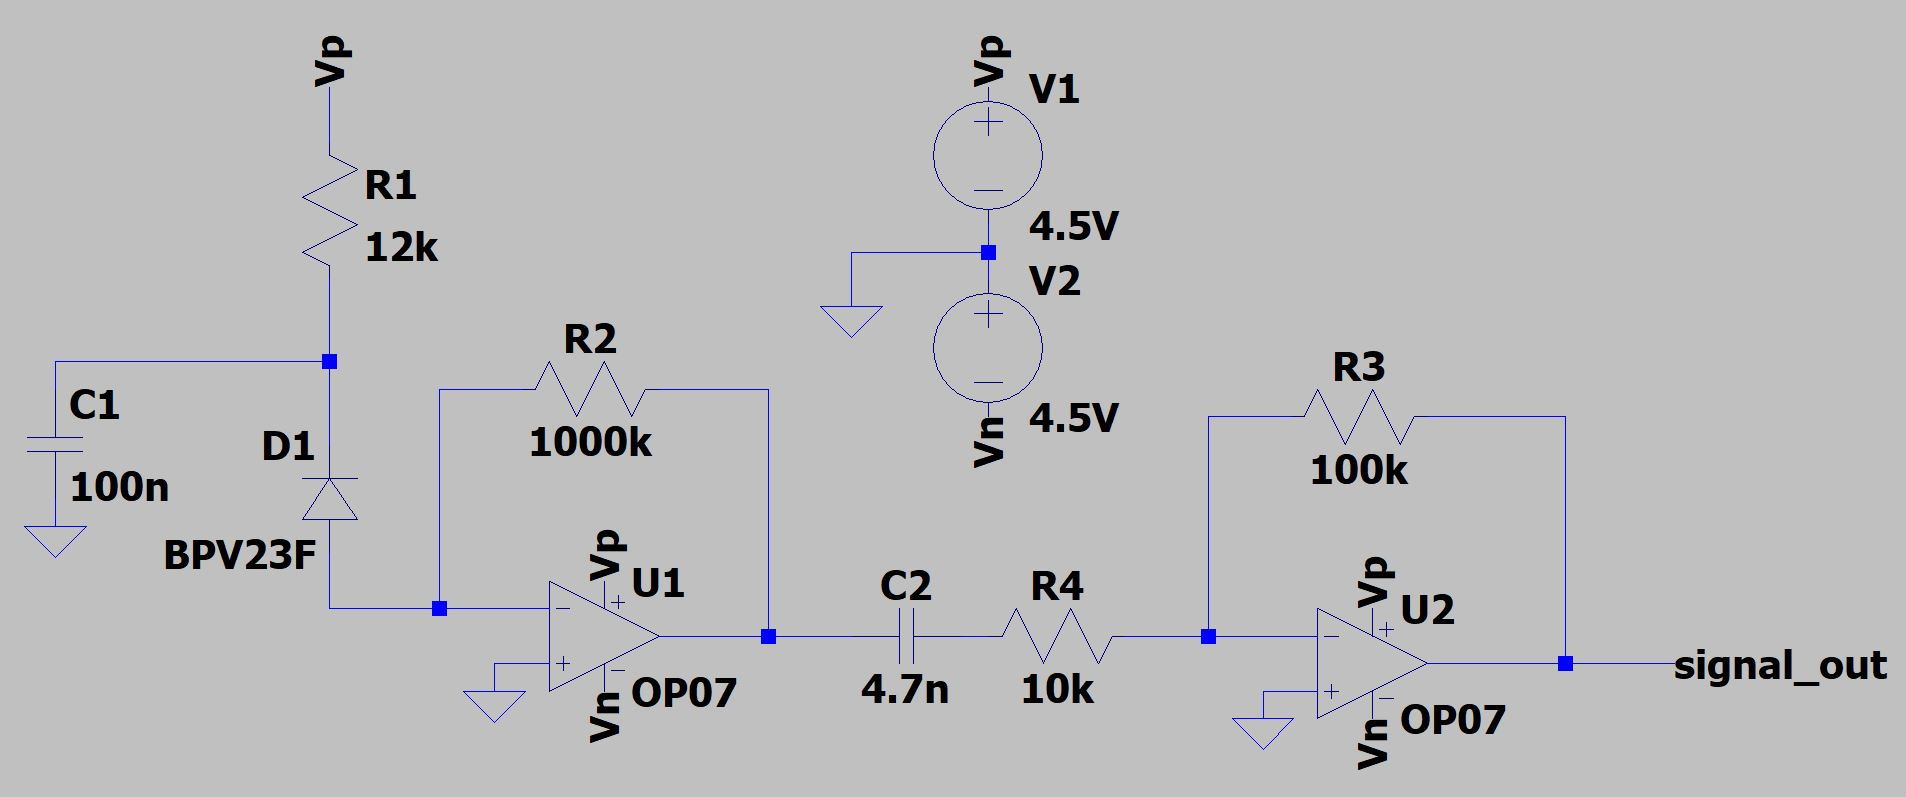
\includegraphics[width=.8\textwidth]{figures/design/photodiode_transimpedance.JPG}
	\caption{Photodiode IR Detector Module Schematic}
	\label{fig:schematic_photodiode_transimpedance}
\end{figure}

\subsubsection{Circuit Design}
A reverse bias voltage is applied across the photodiode to increase its sensitivity. Amplification of the light-induced current is performed through the implementation of a trans-impedance amplifier. A large $1M\Omega$ resistance is used for R2 to maximize the sensitivity and signal to noise ratio.

A second amplification stage is used to further amplify the voltage signal and a decoupling capacitor is used to remove the DC component of the signal before this second stage of amplification.


\subsubsection{Module Realization}
The strip-board implementation of the module is shown in figure \ref{fig:module_photodiode_receiver} below.

\begin{figure}[H]
	\centering
	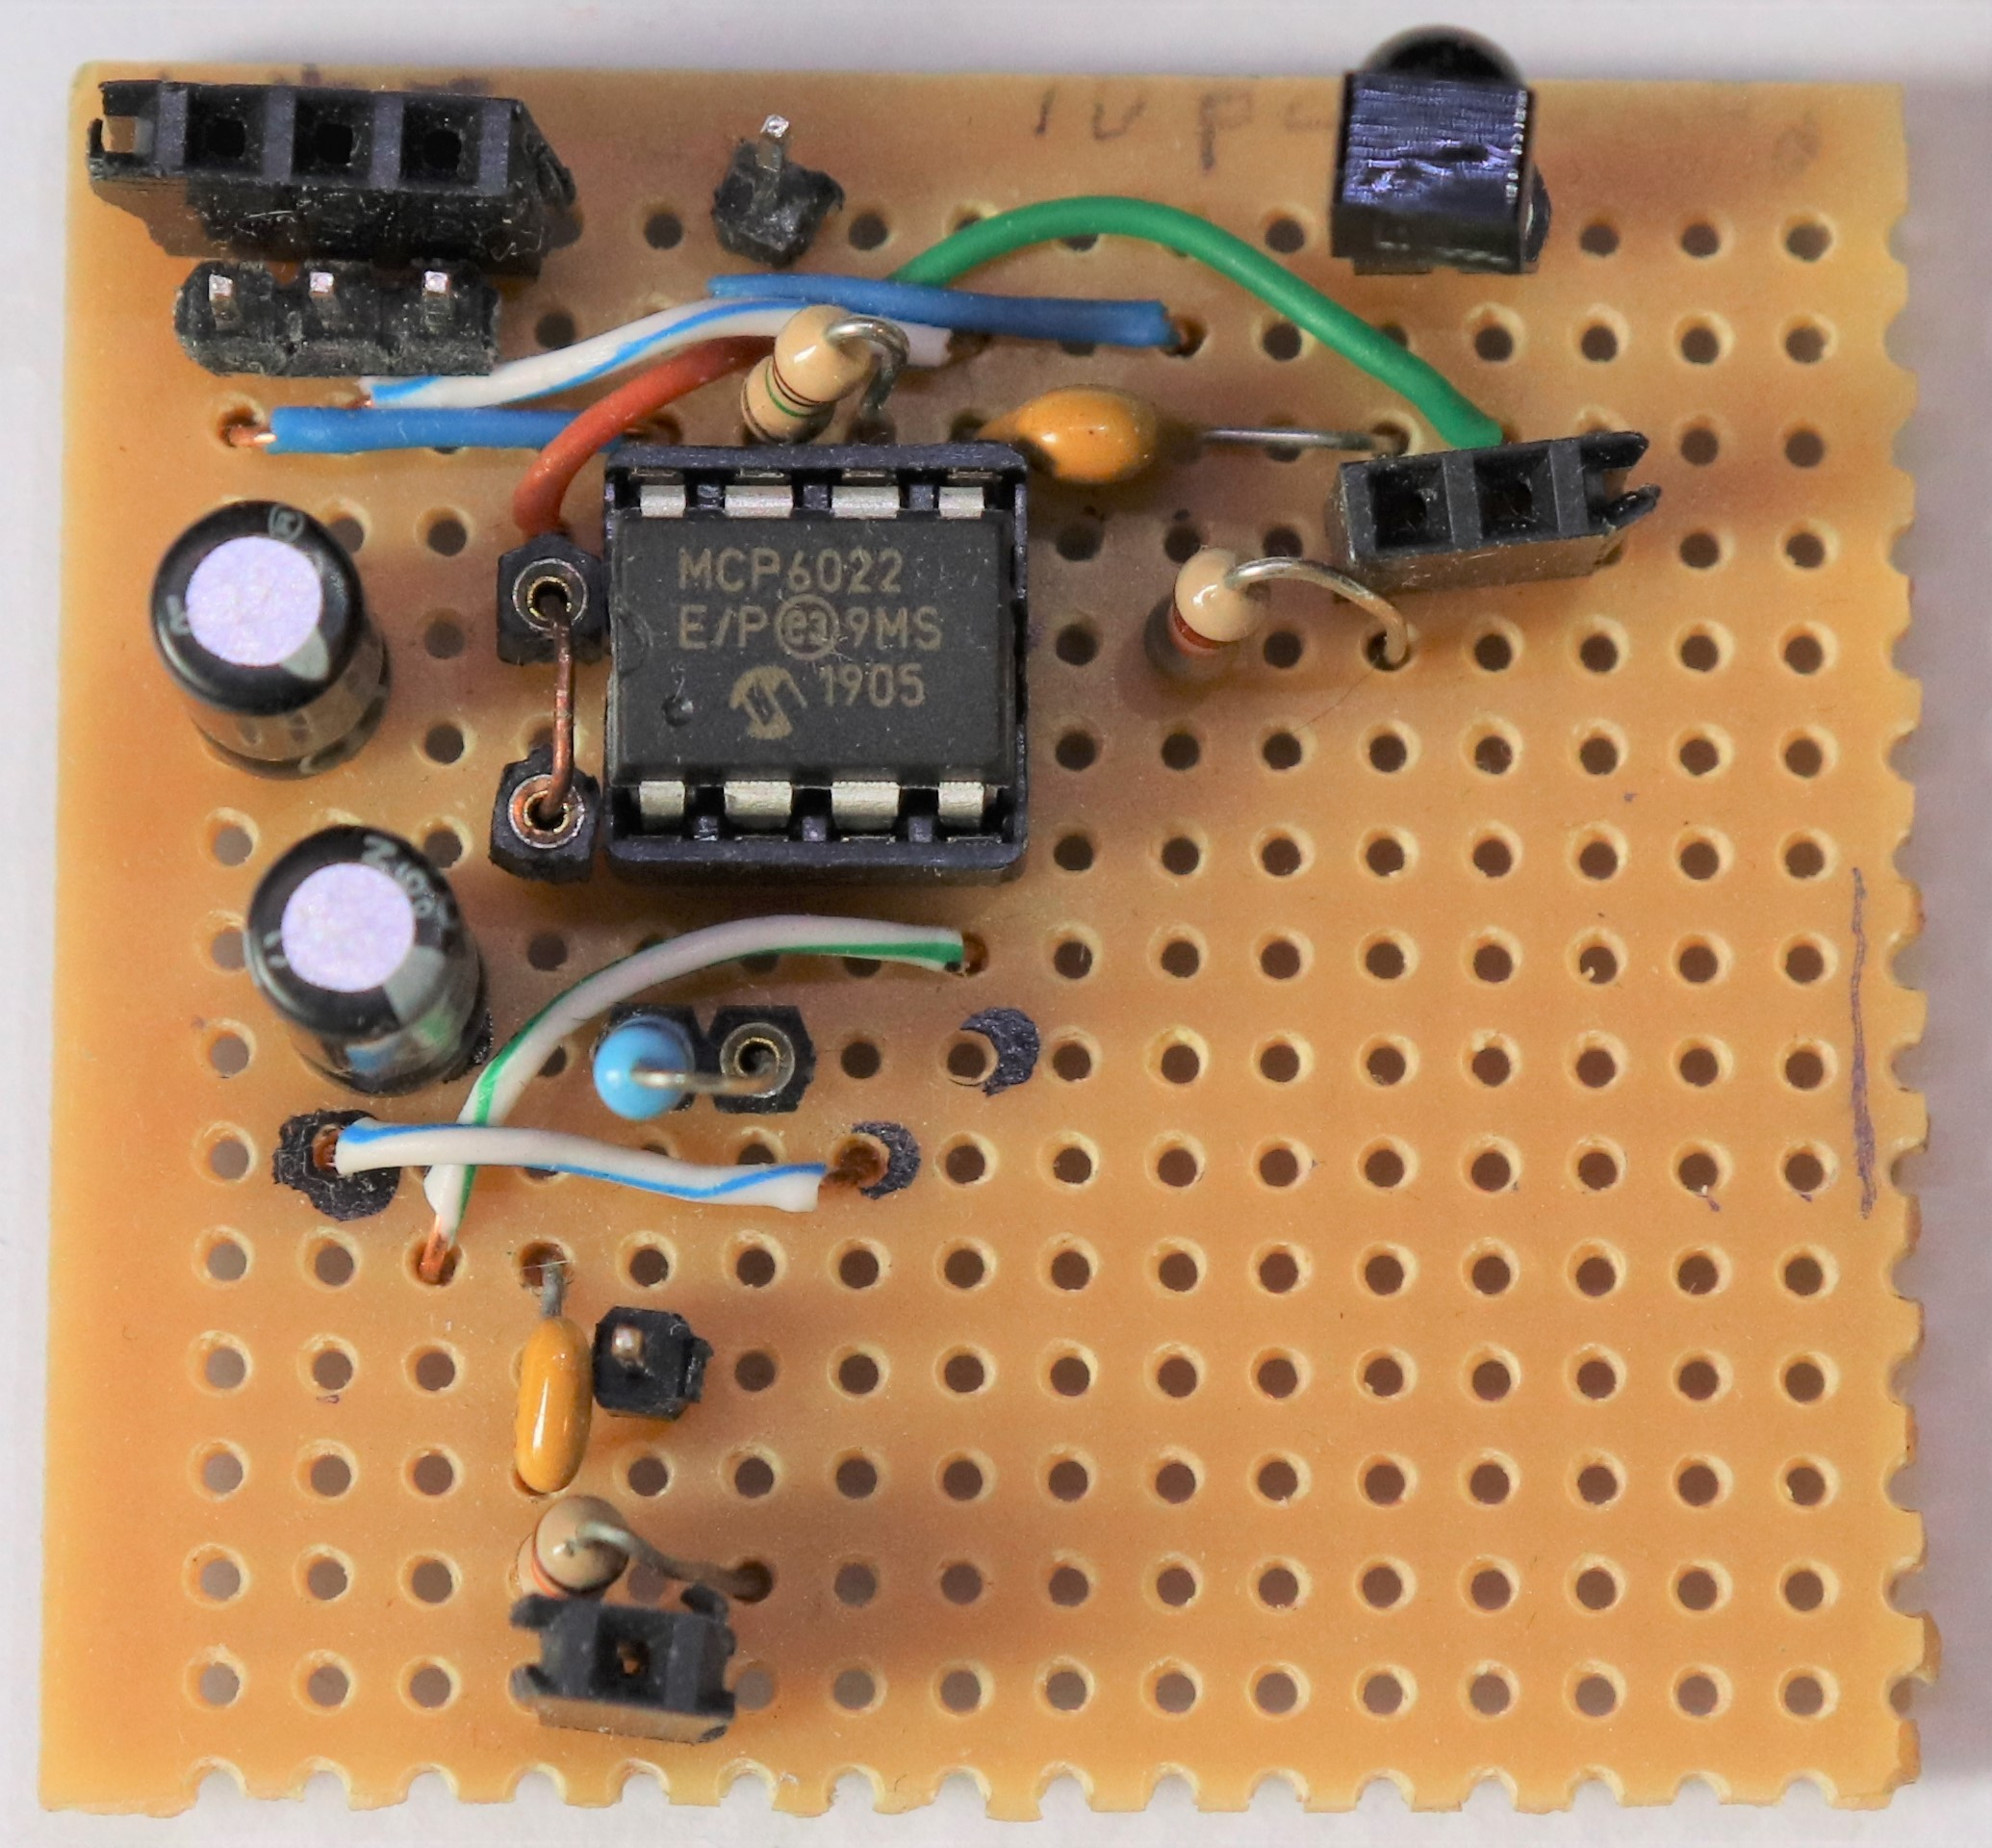
\includegraphics[width=.6\textwidth]{figures/modules/photodiode_receiver.jpg}
	\caption{Photodiode IR Receiver Module}
	\label{fig:module_photodiode_receiver}
\end{figure}


%%%%%%%%%%%%%%%%%%%%%%%%%%%%%%%%%%%%%%%%%%%%%%%%%%%%%%%%%%%



\subsection{Phototransistor IR Detector}

\subsubsection{Functional Design}
The phototransistor IR detector module, like the photodiode IR detector module, is designed to convert fluctuation in infrared radiation into a voltage signal. The circuit is designed to produce an output voltage proportional to changes in the current flowing through the phototransistor.

\subsubsection{Schematic}
Figure \ref{fig:schematic_phototransistor_detector} below shows the schematic for this module.

\begin{figure}[H]
	\centering
	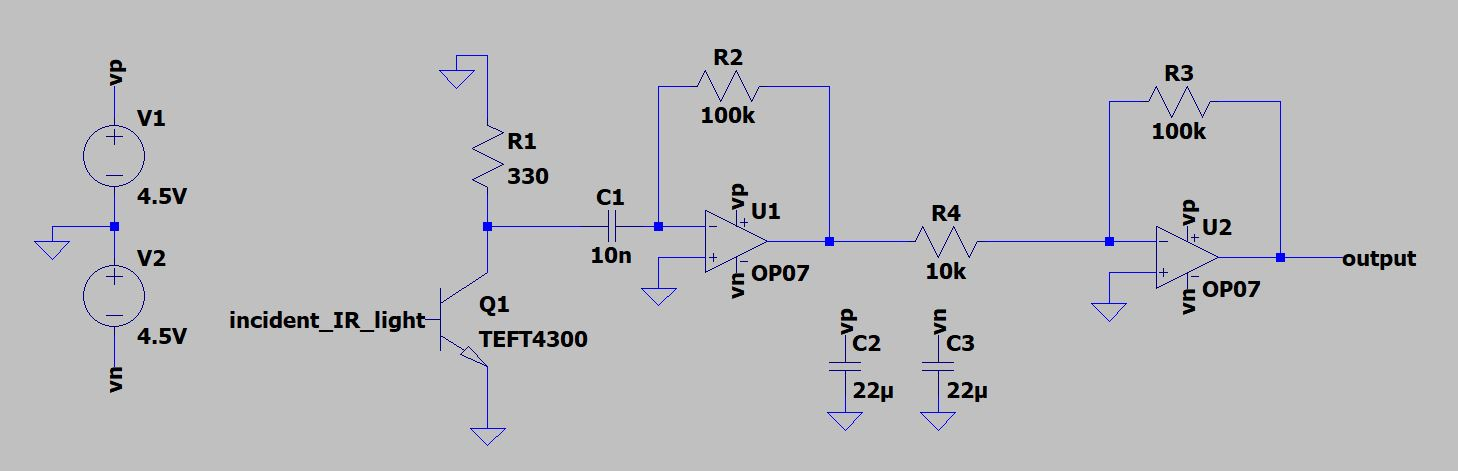
\includegraphics[width=.9\textwidth]{figures/design/phototransistor_detector.JPG}
	\caption{Phototransistor IR Detector Module Schematic}
	\label{fig:schematic_phototransistor_detector}
\end{figure}

\subsubsection{Circuit Design}
The phototransistor is connected to the positive supply rail in series with a $330\Omega$ resistor. The resulting voltage drop induced across the collector-emitter of the phototransistor is proportional to the intensity of incident IR light. This voltage is connected to a set of amplification stages through a decoupling capacitor to remove the signals DC component. Two inverting amplifiers are used to boost the voltage signal.


\subsubsection{Module Realization}
The strip-board implementation of the module is shown in figure \ref{fig:module_photodiode_receiver} below.

\begin{figure}[H]
	\centering
	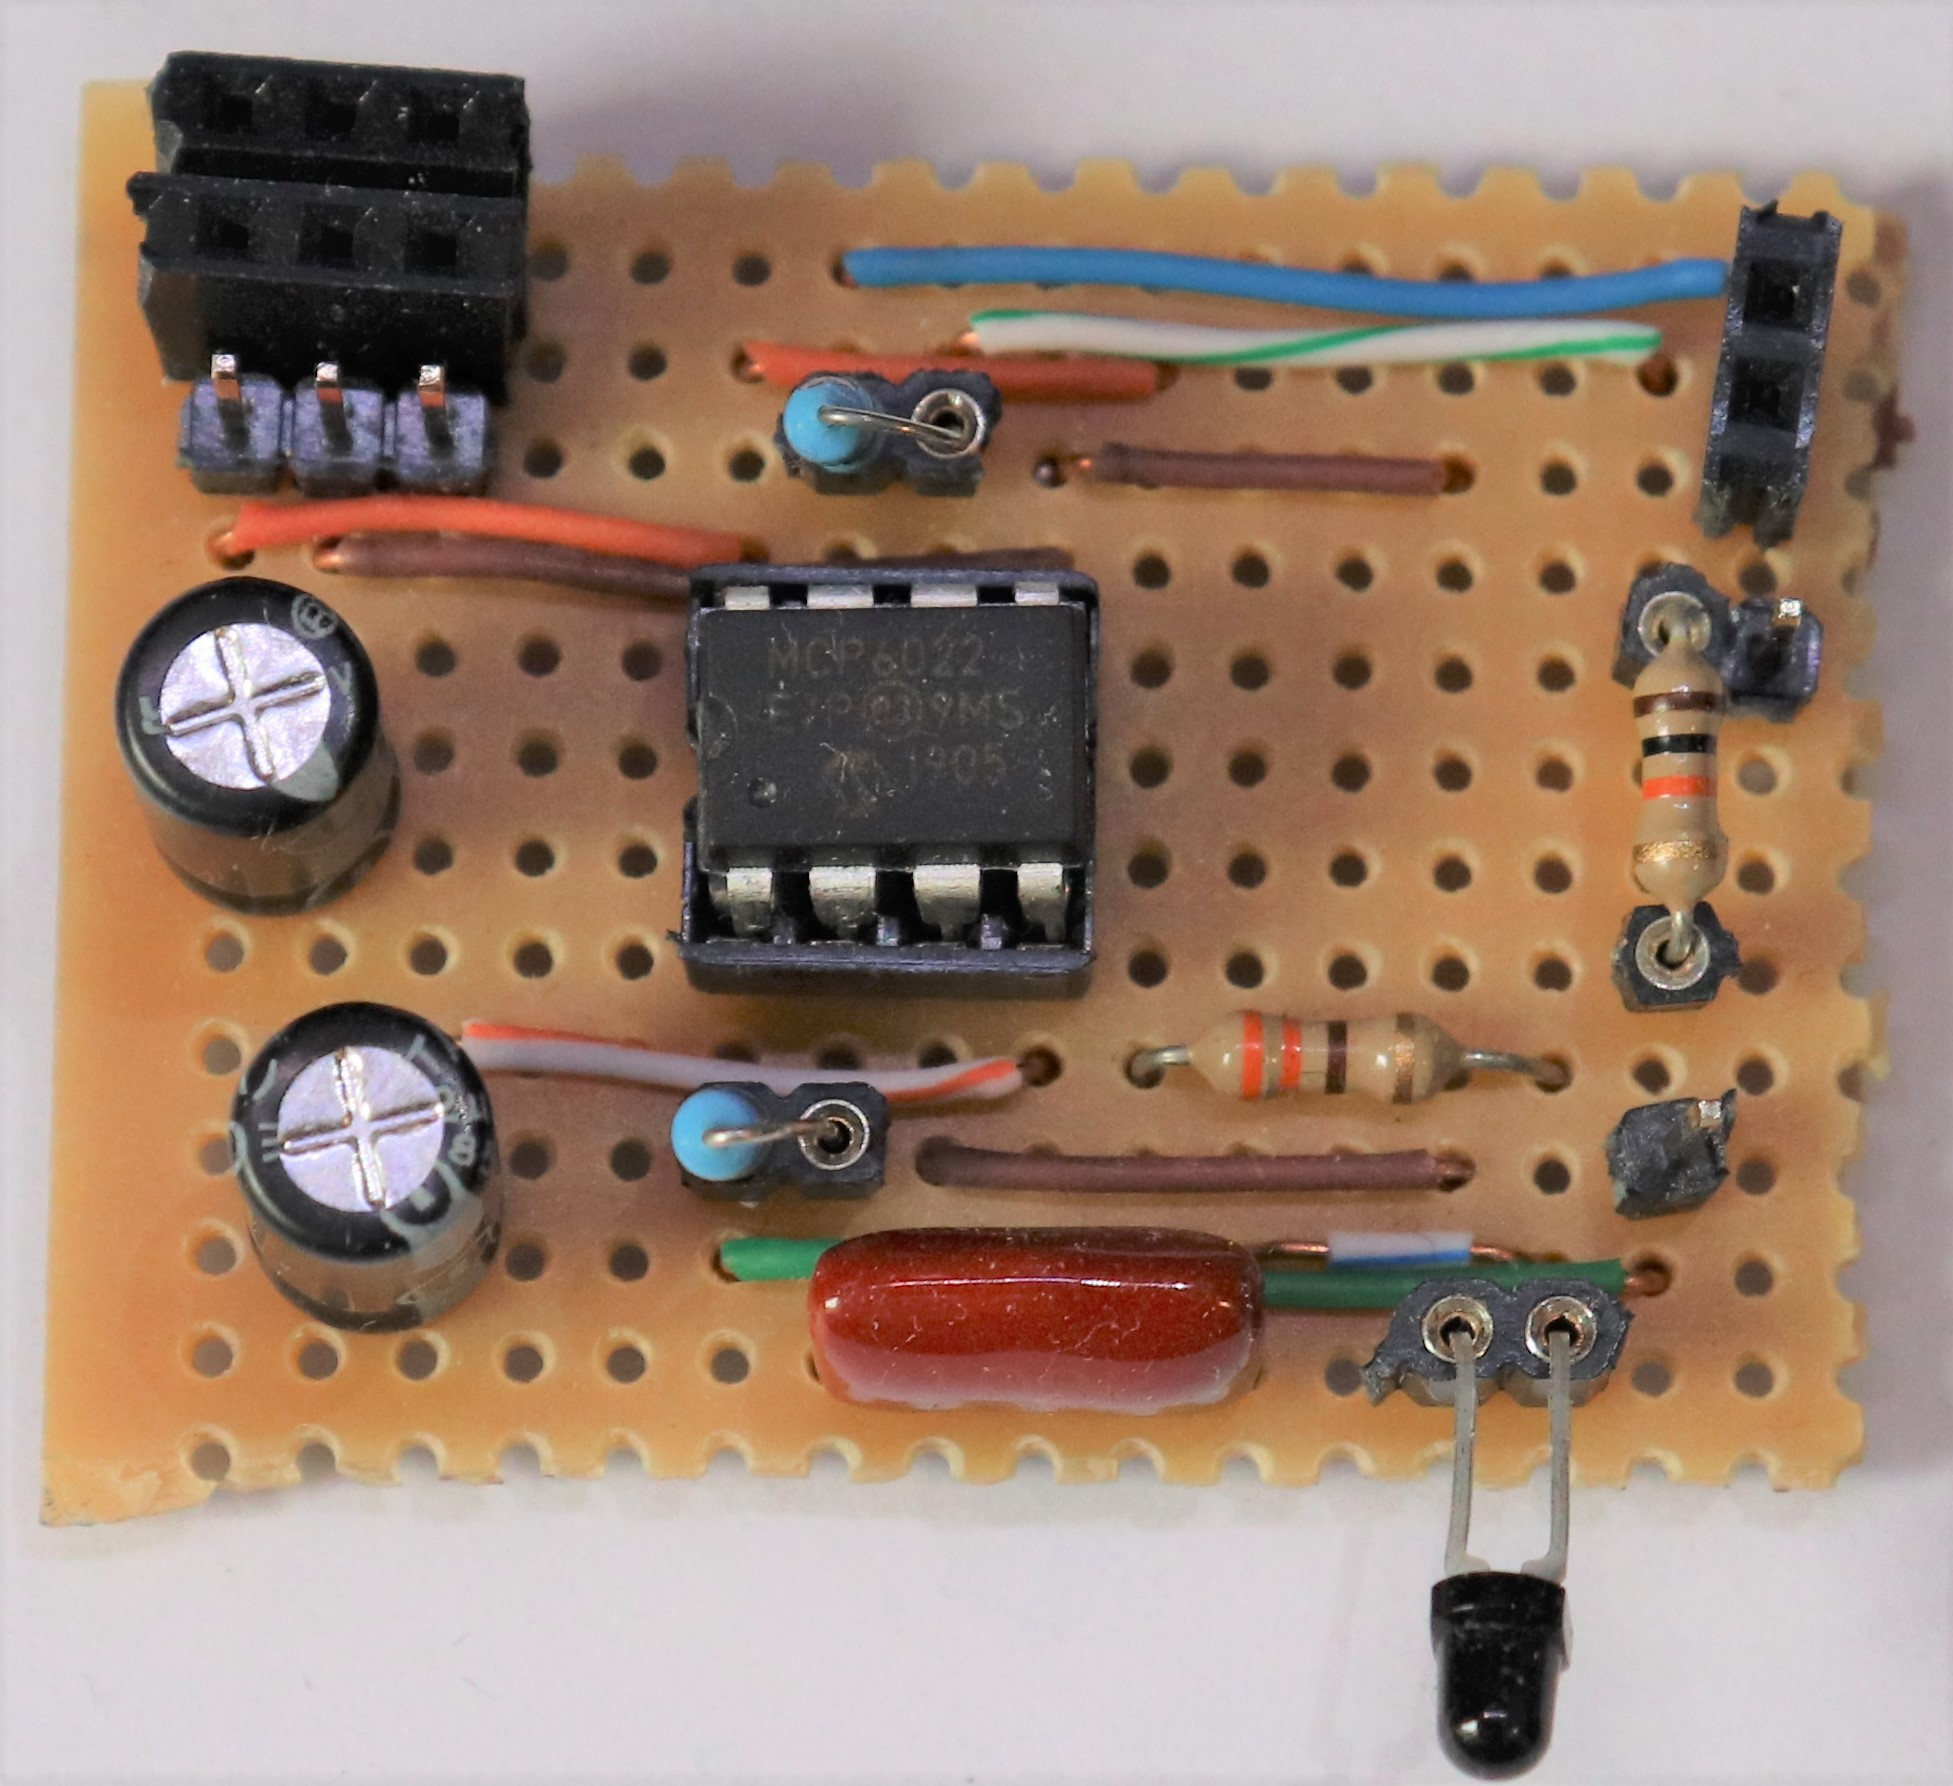
\includegraphics[width=.6\textwidth]{figures/modules/phototransistor_receiver.jpg}
	\caption{Phototransistor IR Detector Module}
	\label{fig:module_phototransistor_detector}
\end{figure}




%%%%%%%%%%%%%%%%%%%%%%%%%%%%%%%%%%%%%%%%%%%%%%%%%%%%%%%%%%%




\subsection{IR Receiver}

\subsubsection{Functional Design}
The IR receiver is an 'all in one package' detector IC designed to detect the presence of a carrier signal in the IR light incident on the detector. The output of the module is high when no modulation is detected and pulled low when modulation is detected.

The module is designed to be powered from a 5V supply, however, the output voltage has been clamped down to 3V to be compatible with the STM32 GPIO pins.

\subsubsection{Schematic}
Figure \ref{fig:schematic_voltage_clamp} below shows the schematic for the voltage clamp used to regulate the output of the TSOP382. The \href{https://www.vishay.com/docs/82491/tsop382.pdf}{datasheet} contains a block diagram (shown in figure \ref{fig:tsop382_block_diagram}) which gives a functional overview of the internal circuitry for this IC.


\begin{figure}[H]
	\centering
	\begin{minipage}{.5\textwidth}
		\centering
		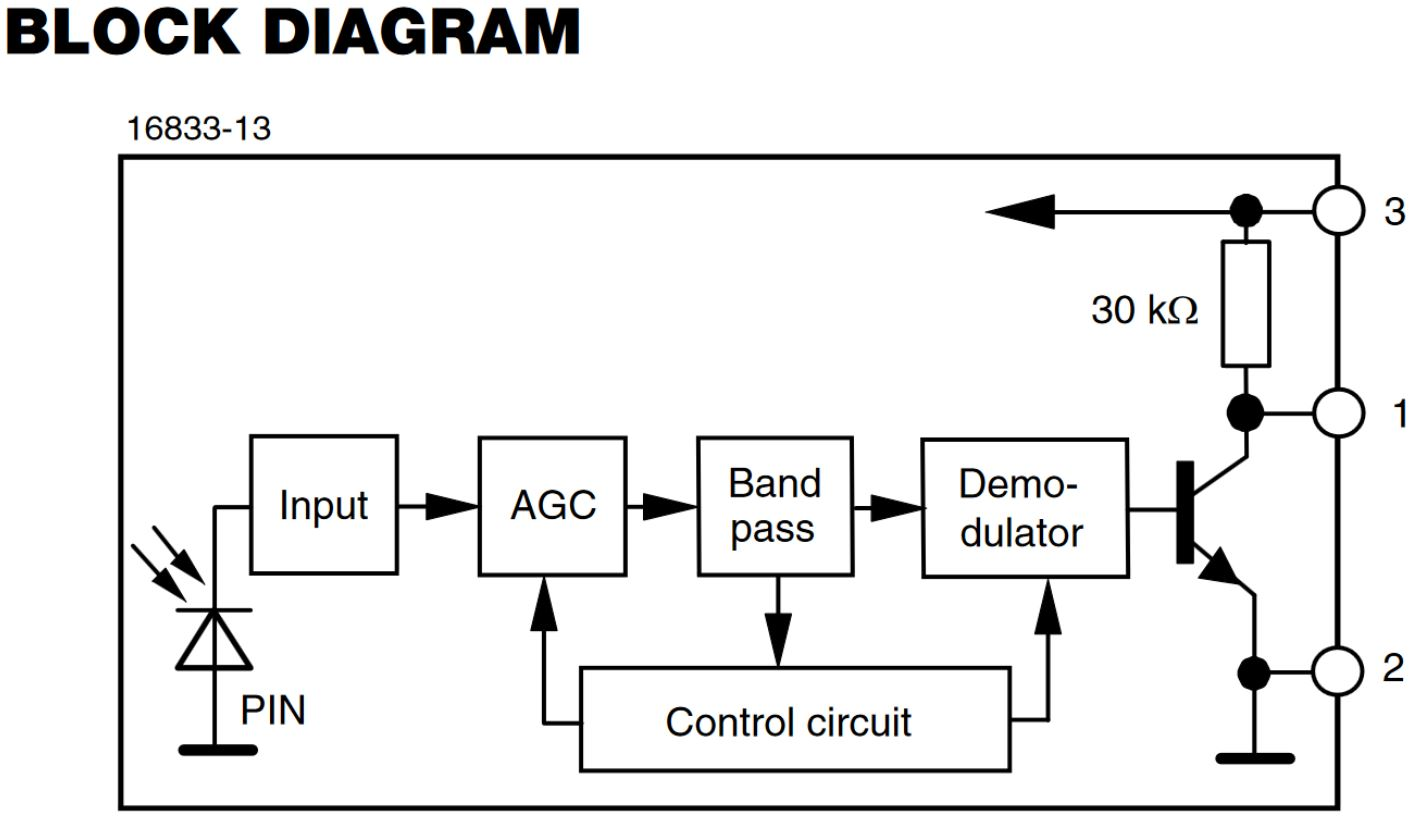
\includegraphics[width=.8\linewidth]{figures/design/TSOP382_block_diagram}
		\captionof{figure}{TSOP382 Functional Diagram}
		\label{fig:tsop382_block_diagram}
	\end{minipage}%
	\begin{minipage}{.5\textwidth}
		\centering
		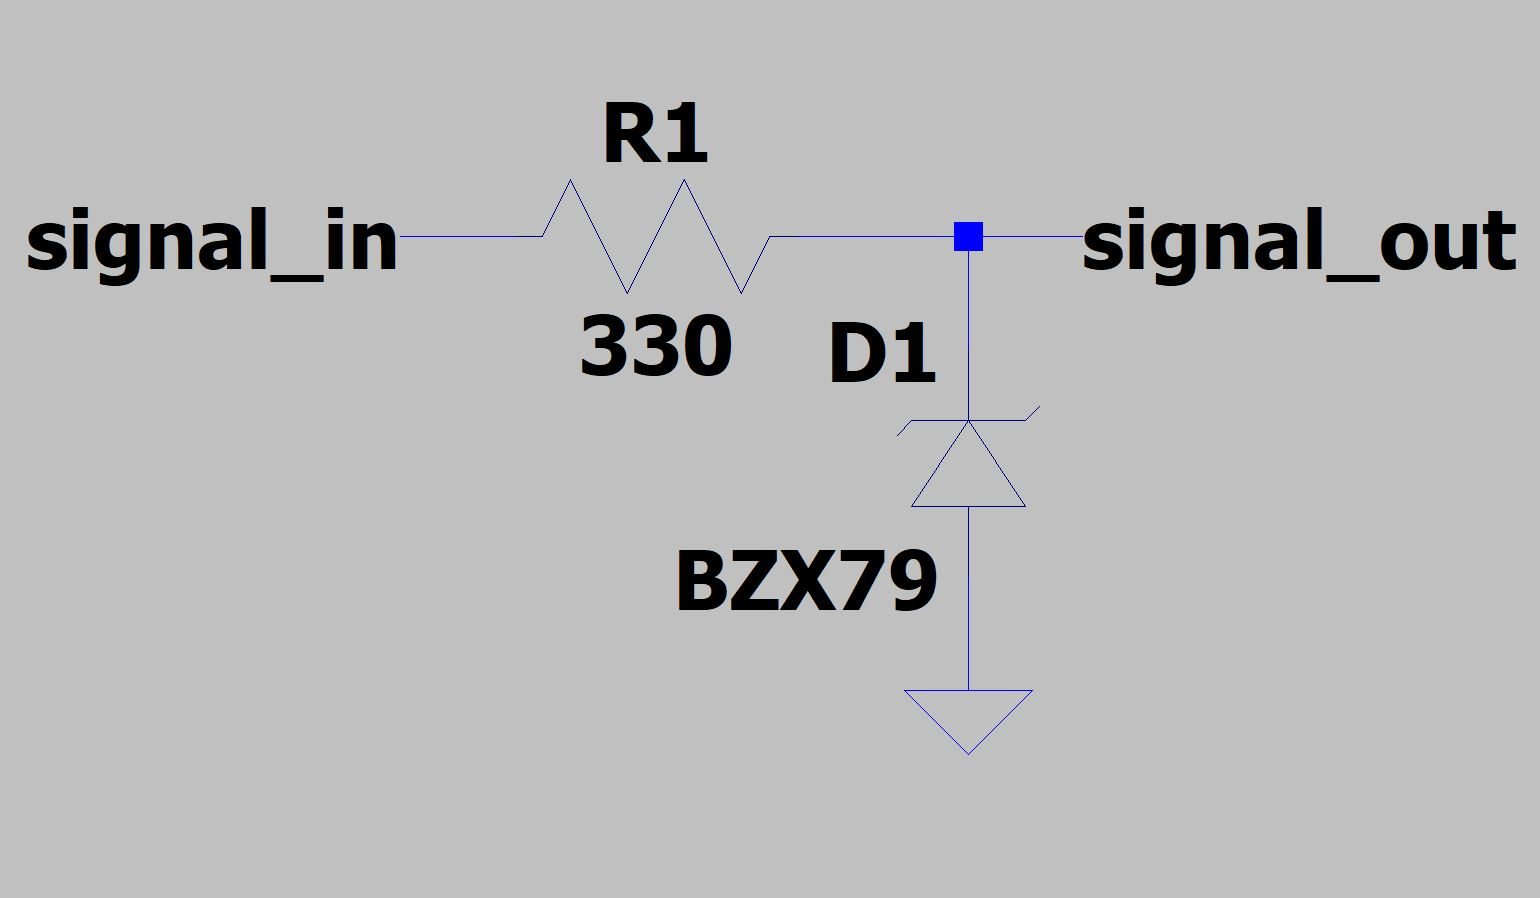
\includegraphics[width=.8\linewidth]{figures/design/over_voltage_protection}
		\captionof{figure}{Voltage Clamp}
		\label{fig:schematic_voltage_clamp}
	\end{minipage}
\end{figure}

\subsubsection{TSOP382}

The TSOP382 IR receiver was chosen due for its low cost, availability and wide range of angles from which it can detect IR radiation. The purpose of this device is to act as a comparison with which to compare the photodiode and phototransistor IR detector modules.


\subsubsection{Module Realization}
The strip-board implementation of the module is shown in figure \ref{fig:module_ir_receiver} below.

\begin{figure}[H]
	\centering
	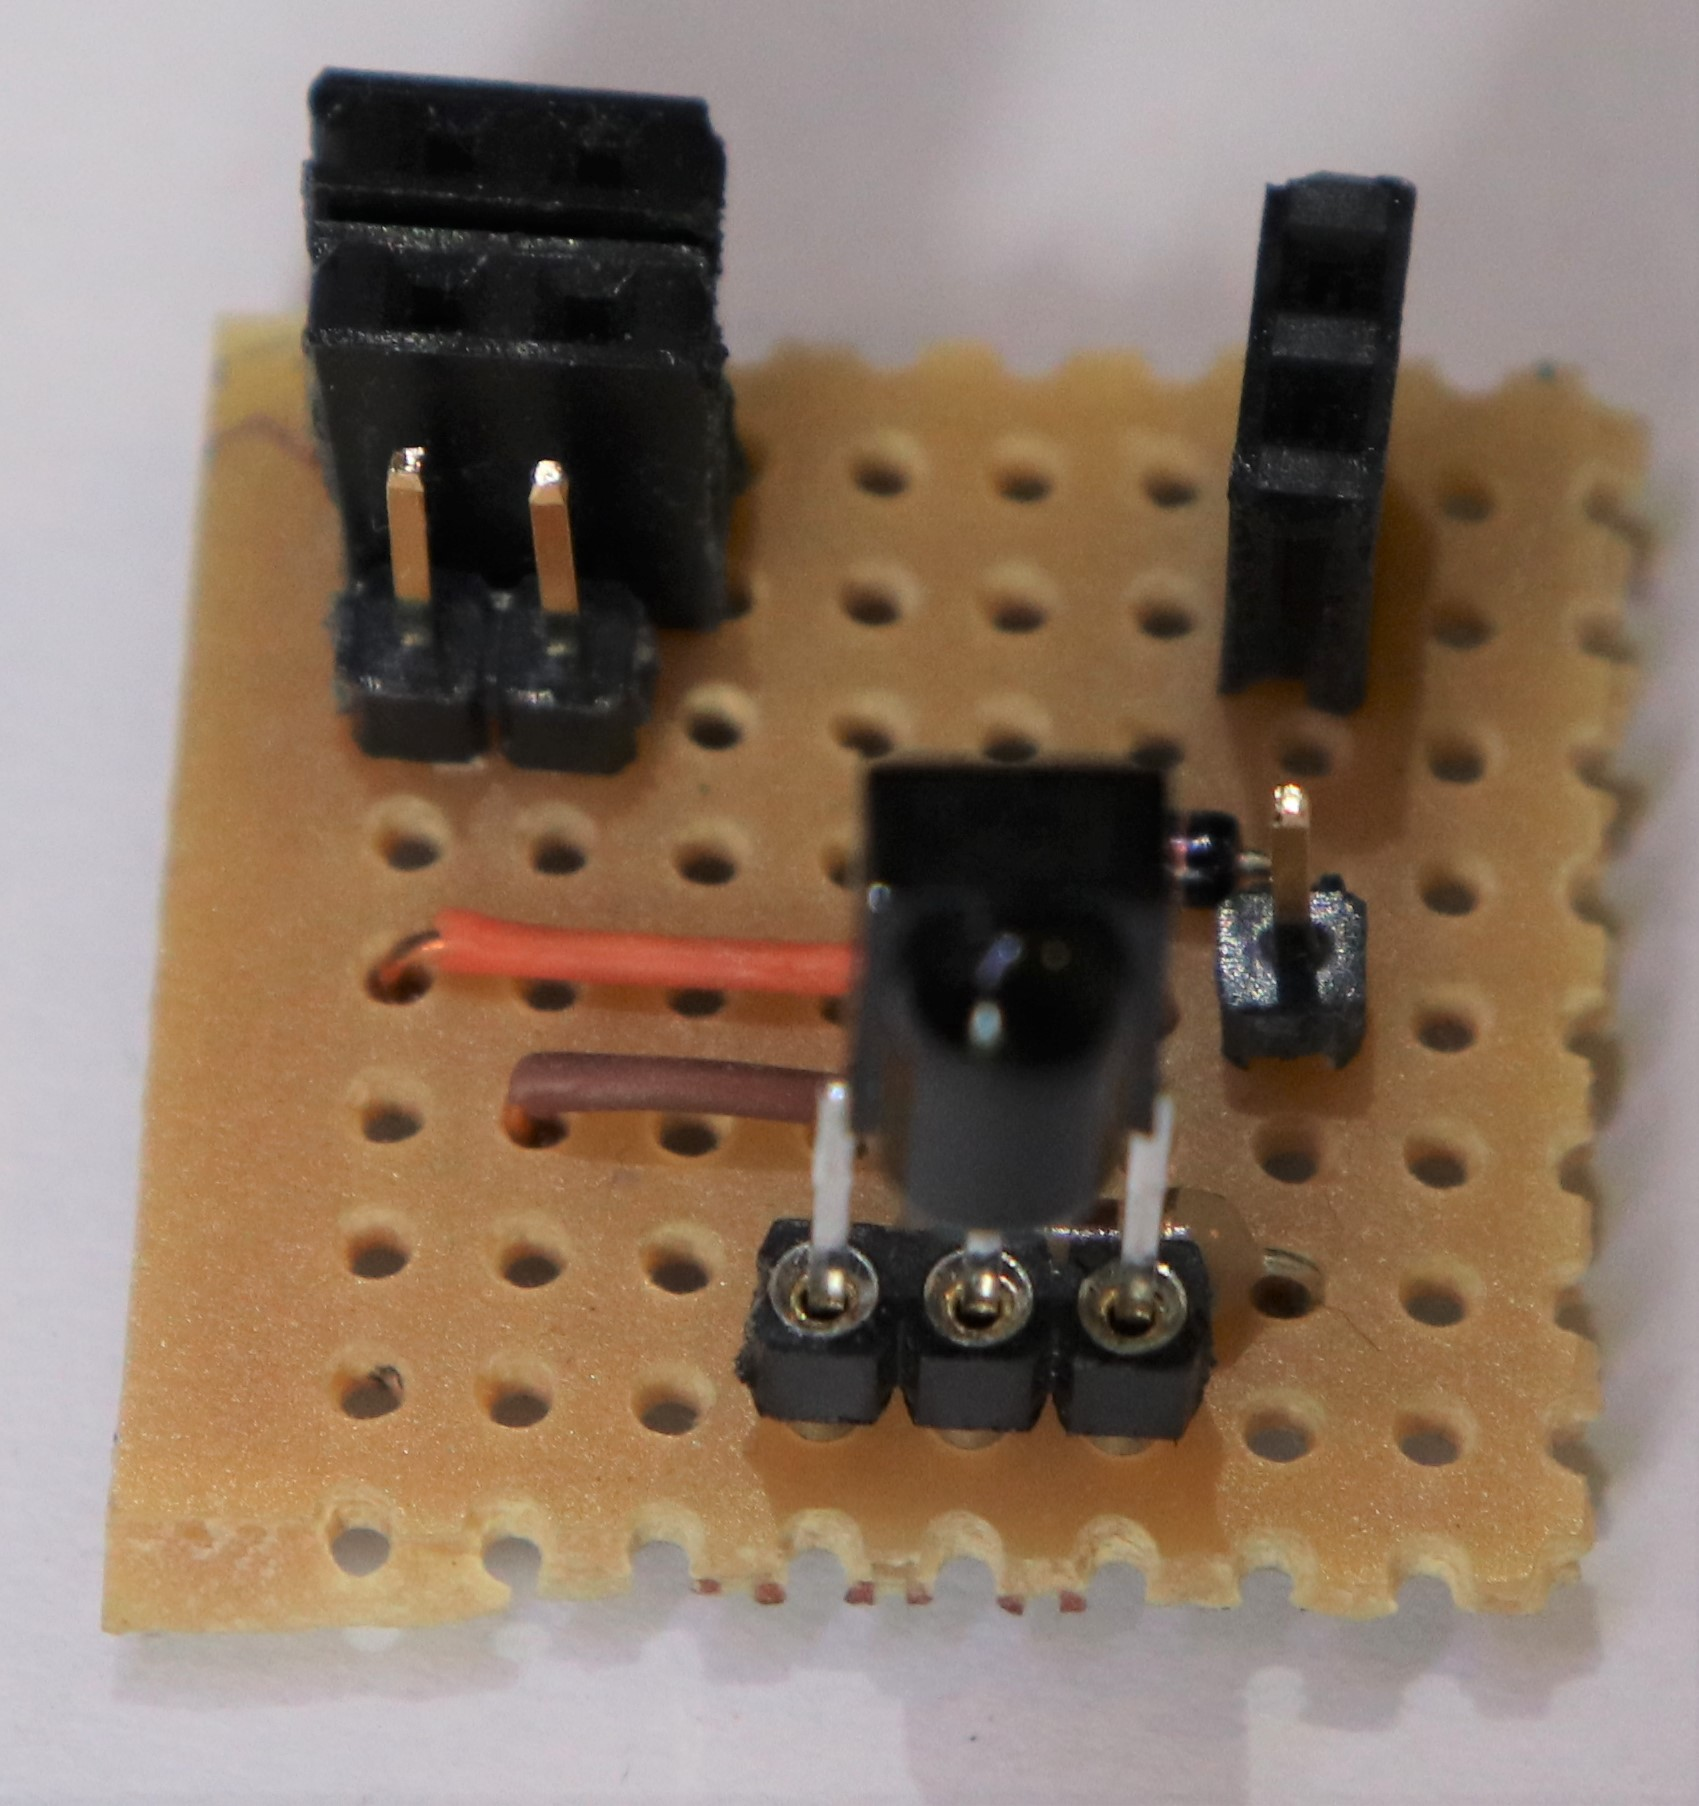
\includegraphics[width=.6\textwidth]{figures/modules/ir_receiver.jpg}
	\caption{IR Receiver Module}
	\label{fig:module_ir_receiver}
\end{figure}



%%%%%%%%%%%%%%%%%%%%%%%%%%%%%%%%%%%%%%%%%%%%%%%%%%%%%%%%%%%



\subsection{Signal Conditioning Module}
\label{sec:signal_conditioning_module}

\subsubsection{Functional Design}
The signal conditioning module is designed to process the output of either the photodiode detector module or phototransistor detector module.

The output of this module is a signal that can be processed by the Goertzel filter. This involves ensuring the output voltage is within the filter's input tolerance and removing any frequencies above the Nyquist sampling rate.

This is performed in three steps. The amplitude of the incoming waveform is reduced, the waveform is filtered and finally, a precision half-wave rectifier is used to rectify the signal.

\subsubsection{Schematic}
Figure \ref{fig:schematic_filter_and_rectify} below shows the schematic for this module.

The module can be broken into two stages as indicated by figure \ref{fig:system_overview_hardware}. The first stage of the module performs filtering and amplitude adjustment. The second stage performs precision rectification.

To prevent the signal conditioning module from interfering with the detector module, the input is passed through a unity buffer. Internally the filtering and rectification stages are also separated by a unity buffer.

\begin{figure}[H]
	\centering
	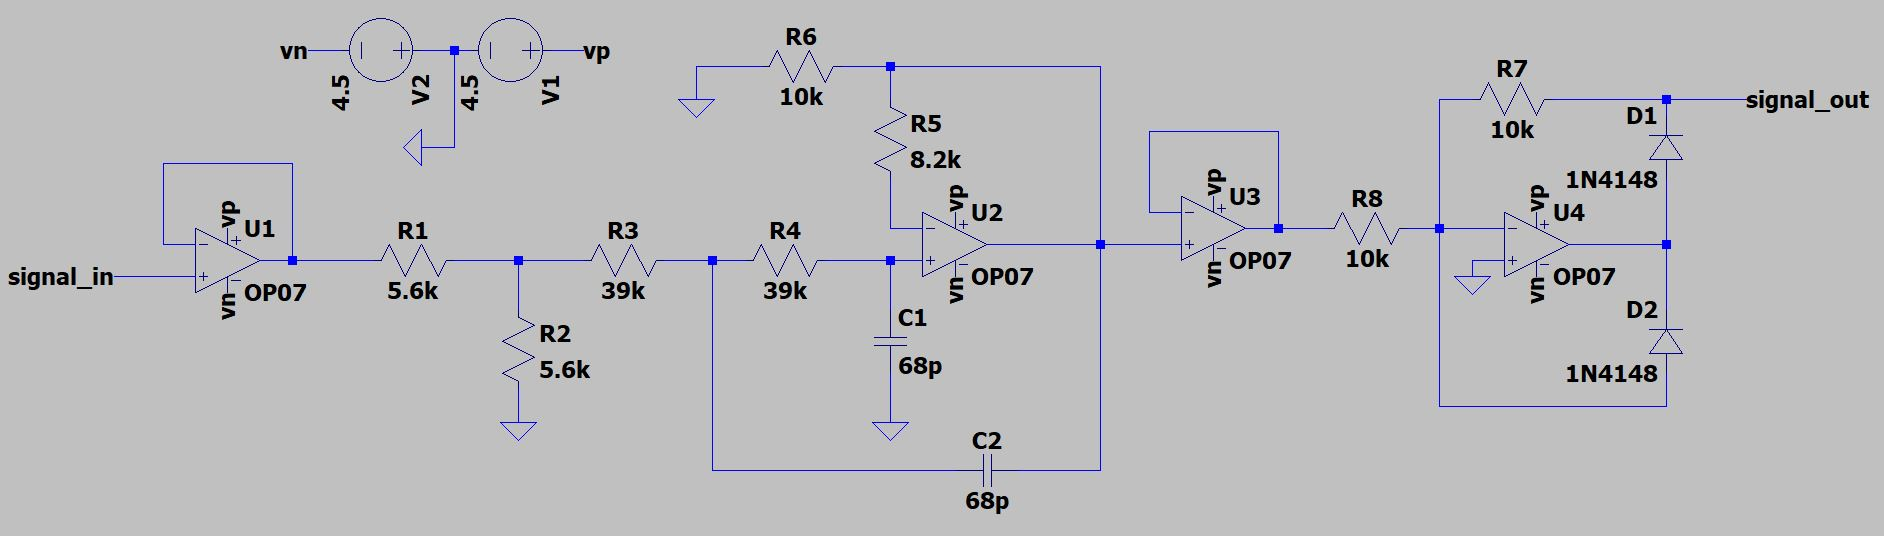
\includegraphics[width=\textwidth]{figures/design/filter_and_rectify}
	\caption{Signal Conditioning Module Schematic}
	\label{fig:schematic_filter_and_rectify}
\end{figure}

The filter implemented is a second-order voltage-controlled voltage source (VCVS) low pass filter in a Chebyshev configuration\footnote{0.5dB passband ripple}. The Chebyshev configuration was chosen because a sharp roll of is desired and because passband ripple will not affect the ability of the Goertzel filter to detect the target frequency.


\subsubsection{Amplitude Adjustment}
The highest amplitude possible for the incoming signal is a square wave with a peak-to-peak value of just under 9V (formed as a result of the amplification stage of the detector module saturating). To ensure the output signal is within the tolerance of the ADC in this extreme case, a voltage divider formed by R1 and R2 before the filter. This divider network halves the amplitude of the incoming signal.

The amplitude is increased slightly due to the gain stage of the filter and this is accounted for by the voltage divider.

\subsubsection{Precision Rectification}

The precision rectifier design is taken from \textit{The art of electronics - 2nd Edition}, see figure \ref{fig:precision_rectifier}. It was chosen for its improved performance, especially at higher frequencies, when compared to more primitive precision rectifiers.

\subsubsection{Filter Design}

The component values where chosen in accordance to the filter design table found on page 274 of the book \textit{The art of electronics - 2nd Edition}\cite{Horowitz1995}. With reference to the schematic (figure \ref{fig:module_filtering_conditioning}), the following relationships hold: \(R_3 = R_4 = R\) and \(C_1 = C_2 = C\).

The desired cut-off frequency is \(f_{c} = 48kHz\), this defines the end of the passband\footnote{Unlike in the case of a Bessel filter, this is not necessarily the -3dB point}.

To achieve a Chebyshev response, the normalization factor and gain are \(f_n = 1.231\) and \(K = 1.842\) respectively.

The gain is set according to the relationship

\[R_5 = (K - 1) \times R_6\].

The values of $R$ and $C$ are determined by the following equation

\[RC = \frac{1}{2\pi f_n f_c}\]

%note the tense change below
Substituting $f_n$ and $f_c$ we find $RC = 2.6935\times 10^{-6}$. It is good practice to select a resistance value between $10k$ and $100k$, the E12 value of $39k\Omega$ was chosen. The corresponding capacitance value is $69pF$, the closest E12 series capacitance value of $68pF$ was used.


\subsubsection{Module Realization}
The strip-board implementation of the module is shown in figure \ref{fig:module_filtering_conditioning} below.

\begin{figure}[H]
	\centering
	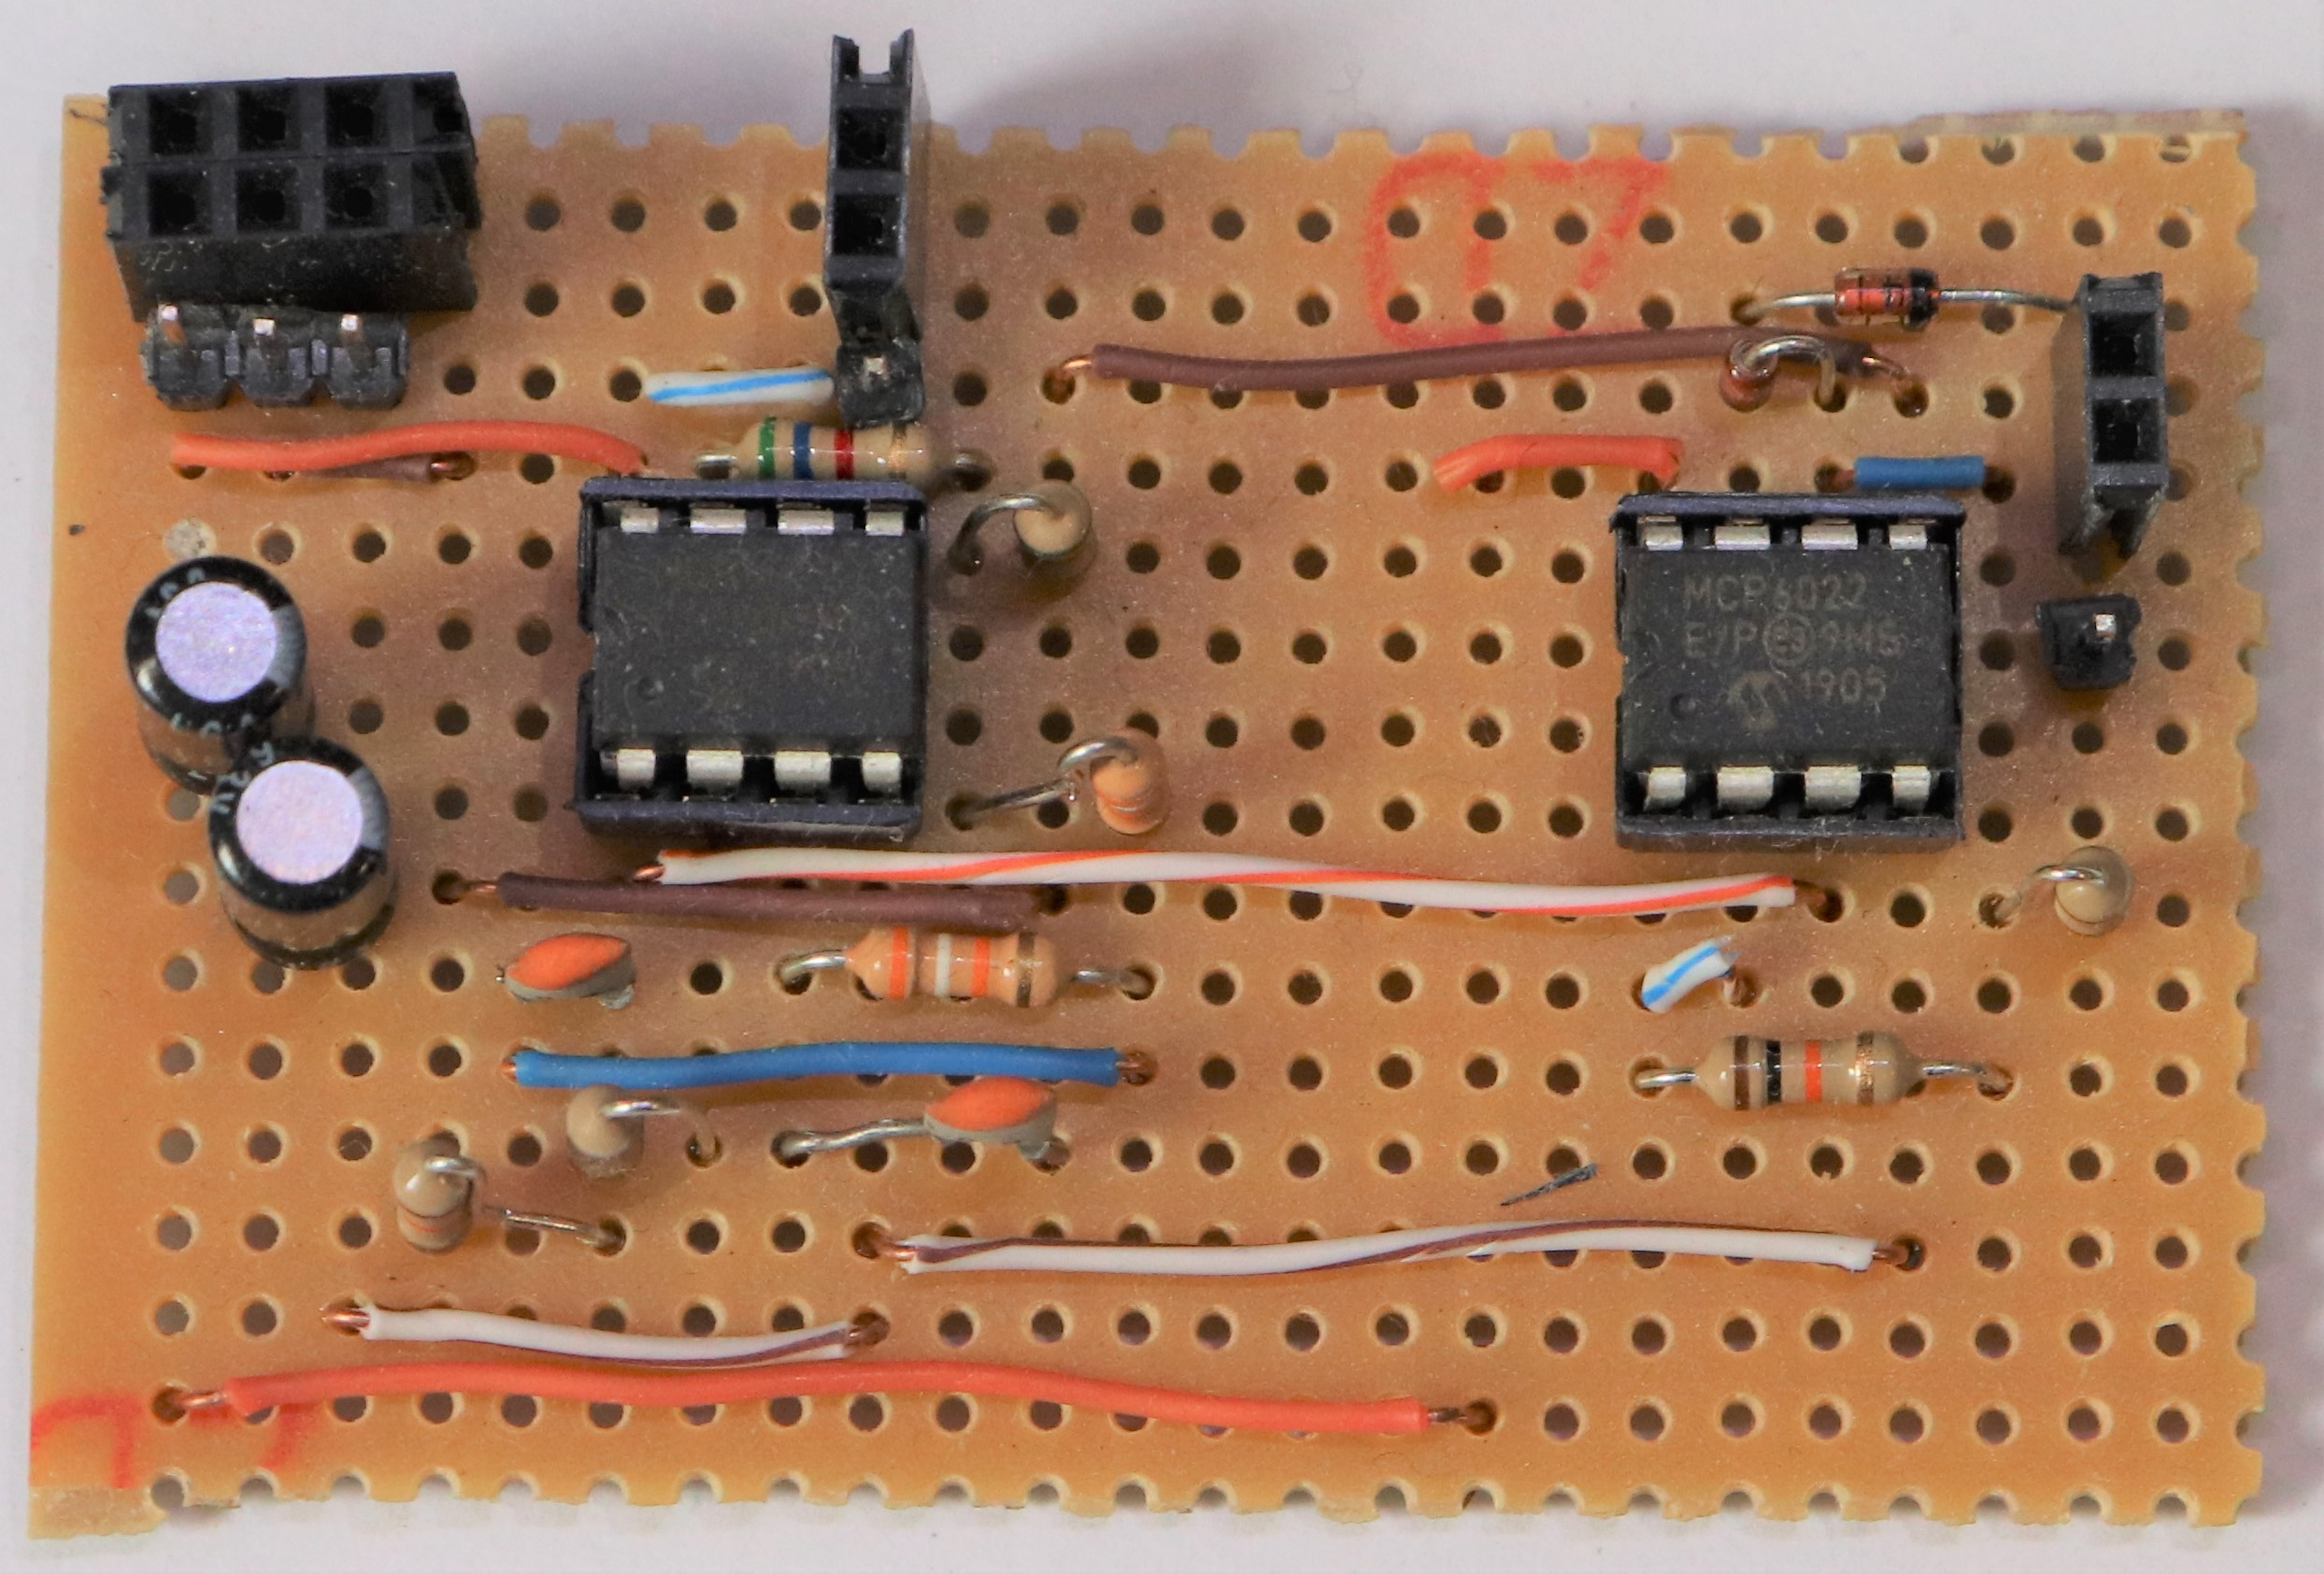
\includegraphics[width=.6\textwidth]{figures/modules/filtering_conditioning.jpg}
	\caption{Signal Conditioning Module}
	\label{fig:module_filtering_conditioning}
\end{figure}

%%%%%%%%%%%%%%%%%%%%%%%%%%%%%%%%%%%%%%%%%%%%%%%%%%%%%%%%%%%




\subsection{Tone Decoder Module}
\label{sec:tone_decoder_hardware}

\subsubsection{Functional Design}
The tone decoder module is designed to indicate the presence of a target frequency in an incoming signal. The input signal is an analog waveform between 0V and 3.3V with no frequency components above half of the filters sampling rate of 144kHz.

The filter achieves this functionality by calculating the DFT coefficient of the frequency bin associated with 36kHz for an incoming signal and outputting a high logic level while the value of the coefficient exceeds a preset threshold.

\subsubsection{Schematic}
The tone decoder module's hardware consists of an STM32F051C6 breakout PCB which is mounted on a strip-board along with supporting circuity (external crystal and voltage regulation). An over-voltage protection clamp (see figure \ref{fig:schematic_voltage_clamp}) was placed on pin 17, the analog input. Three signal LED's were wired to pins 18, 19 and 20 to act as status indicators. The filter's output is produced on pin 19.

Figure \ref{fig:goertzel_schematic_block_form} summarizes the hardware components of the Goertzel module.

\begin{figure}[H]
	\centering
	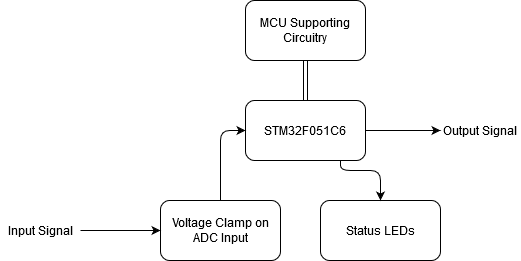
\includegraphics[width=.8\textwidth]{figures/design/goertzel_schematic_block_form.png}
	\caption{Tone Decoder Module - Hardware Breakdown}
	\label{fig:goertzel_schematic_block_form}
\end{figure}

The DSP algorithm is discussed in the software section and can be found in subsection \ref{tone_decoder_software}.

\subsubsection{Module Realization}
The strip-board implementation of the module is shown in figure \ref{fig:module_tone_decoder} below.

\begin{figure}[H]
	\centering
	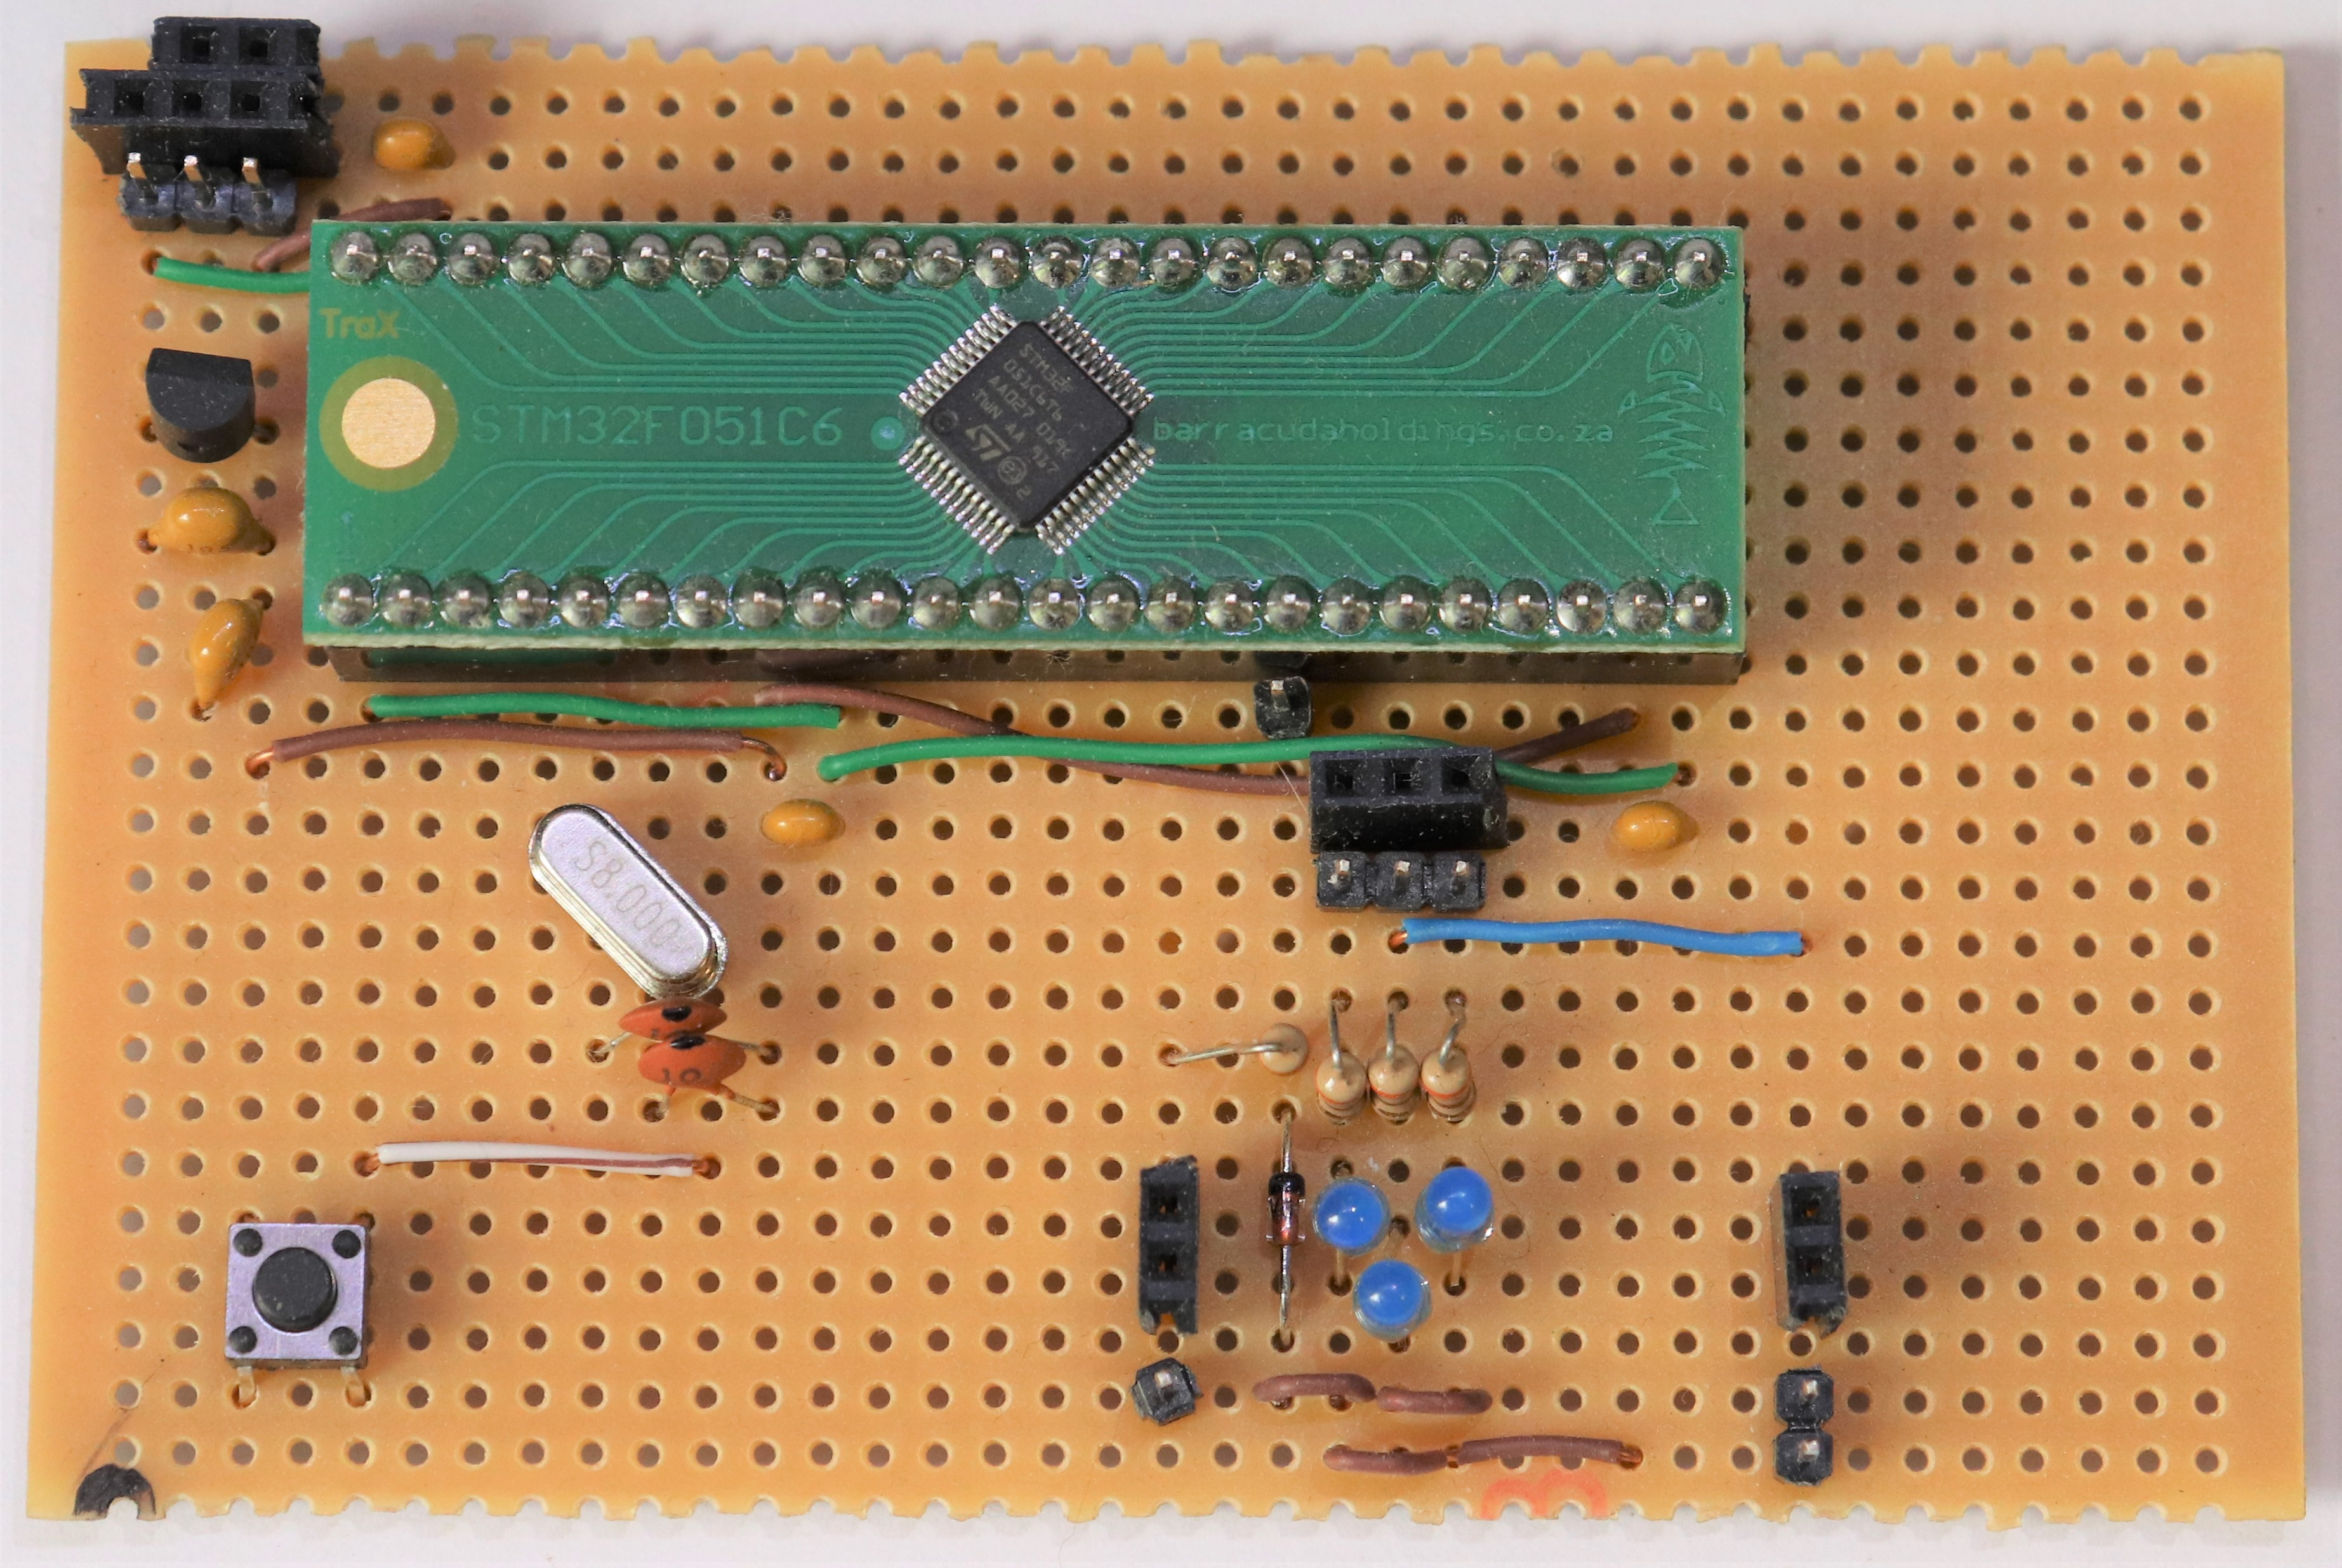
\includegraphics[width=.6\textwidth]{figures/modules/goertzel_filter.jpg}
	\caption{Tone Decoder Module}
	\label{fig:module_tone_decoder}
\end{figure}


%%%%%%%%%%%%%%%%%%%%%%%%%%%%%%%%%%%%%%%%%%%%%%%%%%%%%%%%%%%
%%%%%%%%%%%%%%%%%%%%%%%%%%%%%%%%%%%%%%%%%%%%%%%%%%%%%%%%%%%
\section{Software Design}

\subsection{Tone Decoder}
\label{tone_decoder_software}

The tone decoder is designed to detect the presence of a predefined tone. This is achieved digitally through an implementation of the Goertzel algorithm.

The Goertzel algorithm is presented in section \ref{sec:goertzel_lit_review} and the hardware description for this module is presented in section \ref{sec:tone_decoder_hardware}.

The software design of this module is complex and has been structured in the following way. An overview of the STM32F0 MCU is given to highlight the important features utilized by the tone decoder. Following this is a description of how the Goertzel algorithm is optimized. A section on sampling then presents the constraints associated with the sampling rate and the number of samples required by the algorithm. Finally the practical implementation is documented.


\subsubsection{Overview}
The algorithm is implemented on the STM32F0, a low-cost 32-bit microcontroller that utilizes the ARM Cortex-M0 CPU core. This microcontroller does not contain any dedicated DSP peripherals nor does it contain any hardware dedicated to floating-point arithmetic. Therefore careful consideration must be taken to optimize the performance of the Goertzel filter implementation.

The STM32F0 is equipped with several timers, direct memory access (DMA) and an advanced interrupt controller, these peripherals are indispensable resources for the implementation of the real-time digital filter. Figure \ref{fig:goertzel_functional_diagram} shows the functional blocks for the Goertzel filter. The flow of data is indicated with a solid line and the clocking signals are indicated with a dashed line.

\begin{figure}[H]
	\centering
	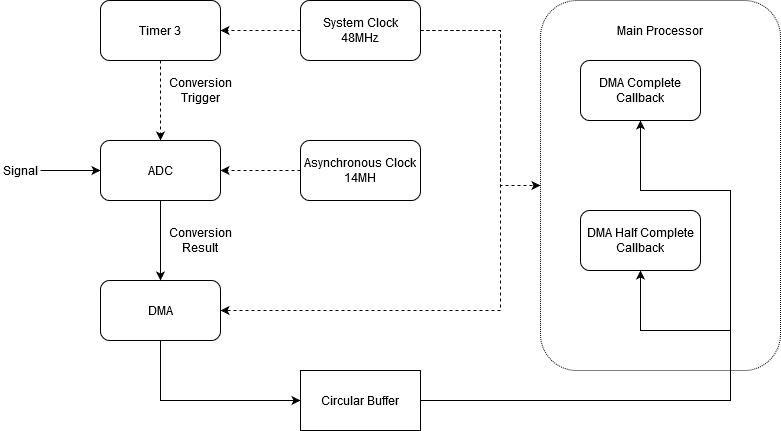
\includegraphics[width=.8\textwidth]{figures/design/goertzel_filter_functional.png}
	\caption{Goertzel Filter Implementation - Functional Block Diagram}
	\label{fig:goertzel_functional_diagram}
\end{figure}


\subsubsection{Filter Optimization}
\label{sec:filter_optimization_design}
The Goertzel filter is optimized in two different ways. The first optimization involves configuring the timer, ADC and DMA to continuously sample the incoming signal and store the conversion results in a circular buffer. Without these peripherals, it would not be possible to perform filtering in real-time.

The second means of optimization requires manipulating the algorithm's parameters to reduce the number of multiplications. Section \ref{sec:goertzel_parameters} presents these parameters. By manipulating $omega$ to equal $\frac{\pi}{2}$, the algorithm constants $cosval$ and $sinval$ can be made equal to zero and one respectively. Thus reducing line 13 of listing \ref{lst:goertzel_algorithm} to $s0 = samples(i) - s2$. 

Even after these optimizations the STM32F0 is not fast enough to process every sample. This is solved by sampling twice as many samples, but only using the first N samples to calculate the DFT coefficient. This works because the sections of waveform that go unprocessed are much shorter than the tone duration.

\subsubsection{Sampling}
\label{sec:sampling_frequency_constraints}
The sampling frequency determines the highest frequency component that may be present in a sampled waveform before aliasing will occur.

A higher sampling rate increases the bandwidth of the Goertzel filter and relaxes the requirements for the anti-aliasing filter (see section \ref{sec:signal_conditioning_module}), however the sampling frequency is limited by the speed of the microcontroller.
A hard upper limit is imposed by the physical limitations of the ADC and DMA peripherals and a soft upper limit is imposed by the rate at which samples can be processed by the CPU.
%It is therefore desirable to select a lower sampling rate.

In addition to the sampling frequency, the number of samples (N) processed by the Goertzel algorithm determines the frequency response of the filter. For a constant sampling rate, decreasing N lowers the resolution of each frequency bin causing the tone detector to trigger on a wider band of frequencies, however increasing N causes the time taken to collect and process the samples to increase. For the filter to be effective, the processing period must be significantly short than the duration of the tone being detected.

\textbf{Omega Value}\\
The value of omega cannot be set directly, rather it's relationship to the target bin frequency and sampling frequency must be established so that by carefully choosing these, the value of omega can be indirectly manipulated.

Line 4 of the algorithm in listing \ref{lst:goertzel_algorithm} provides the relationship between k, N and $\omega$

\begin{equation}
\omega = \frac{2\pi * k}{N}
\end{equation}

Substituting \(\omega = \frac{\pi}{2} + 2\pi m,\; m\epsilon \mathbb{Z}\) and simplifying shows

\begin{equation}
\label{eqn:k_N_constraint}
\frac{k}{N} = \frac{1+4m}{4},\; m\epsilon \mathbb{Z}
\end{equation}

If only integer values for k, N, $f_{sampling}$ and $f_{bin}$ are considered, line 3 of the algorithm provides the relationship between these parameters which may be expressed by the following equation

\begin{equation}
\label{eqn:k_N_and_fb_fs}
\frac{k}{N} = \frac{f_{bin}}{f_{sampling}}
\end{equation}

Equation \ref{eqn:k_N_and_fb_fs} shows that the ratio of $f_{bin}$ to $f_{sampling}$ must be equal to that of k to N. This relationship indicates that the only realisable value for m is zero. Any value of m greater than zero requires a sampling frequency lower than the bin frequency which violates the Nyquist criteria and a negative value of m would require (for $f_{bin} \approx 36kHz$) a negative sampling frequency which is nonsensical. The final relationship between the ratios is summarised in equation \ref{eqn:k_N_and_fb_fs_ratio}.

\begin{equation}
\label{eqn:k_N_and_fb_fs_ratio}
\frac{k}{N} = \frac{f_{bin}}{f_{sampling}} = \frac{1}{4}
\end{equation}

\subsubsection{Practical Implementation}
\textbf{Sampling Frequency}\\
The desired bin frequency is 36kHz, according to equation \ref{eqn:k_N_and_fb_fs_ratio} this requires a sampling frequency of 144kHz. This is within the constraints set out in section \ref{sec:sampling_frequency_constraints}.

The ADC conversions are triggered by timer 3, a general-purpose 16-bit timer. The timer uses a pre-scalar and counter period value. The frequency of the timer's output and as a result the sampling frequency is given by \(f_{sampling} = \frac{f_{system\_clock}}{prescaler \times cperiod}\). Substituting our system clock frequency, desired sampling frequency and rearranging the equation we find the product of the pre-scalar and clock period values.

\[prescaler \times cperiod = \frac{48 \times 10^6}{144 \times 10^3} = 333.\dot{3}\]

The result, $333.\dot{3}$ is irrational, therefore the closest integer value of 333 is used. The resulting sampling frequency is $144.\dot{1}4\dot{4}$ kHz. Revisiting equation \ref{eqn:k_N_and_fb_fs_ratio}, we see that we require $f_{bin} = 36.036$kHz to preserve the ratio required for optimization.

\textbf{Number of Samples - N}\\
Each Goertzel calculation is performed on 16 samples. This number of samples provides a good balance between the bandwidth of the DFT frequency bin and the processing delay.

\textbf{Schmitt-Trigger}\\
The output of the Goertzel filter module is a binary state indicating the presence or absence of a 36kHz frequency. A high output indicates the presence of the specified tone in the sampled waveform.

Based on the simulations performed (see section \ref{sec:results_frequency_response}), the value $6\times 10^{6}$ is selected as the threshold for the squared magnitude of the DFT bin's coefficient. A Schmitt-trigger is implemented to prevent oscillations whenever the squared magnitude of the coefficient is close to the threshold. The output is configured to activate when the value exceeds the threshold by $2\times 10^{6}$ and deactivate when the value is $2\times 10^{6}$ below the threshold.

\begin{figure}[H]
	\centering
	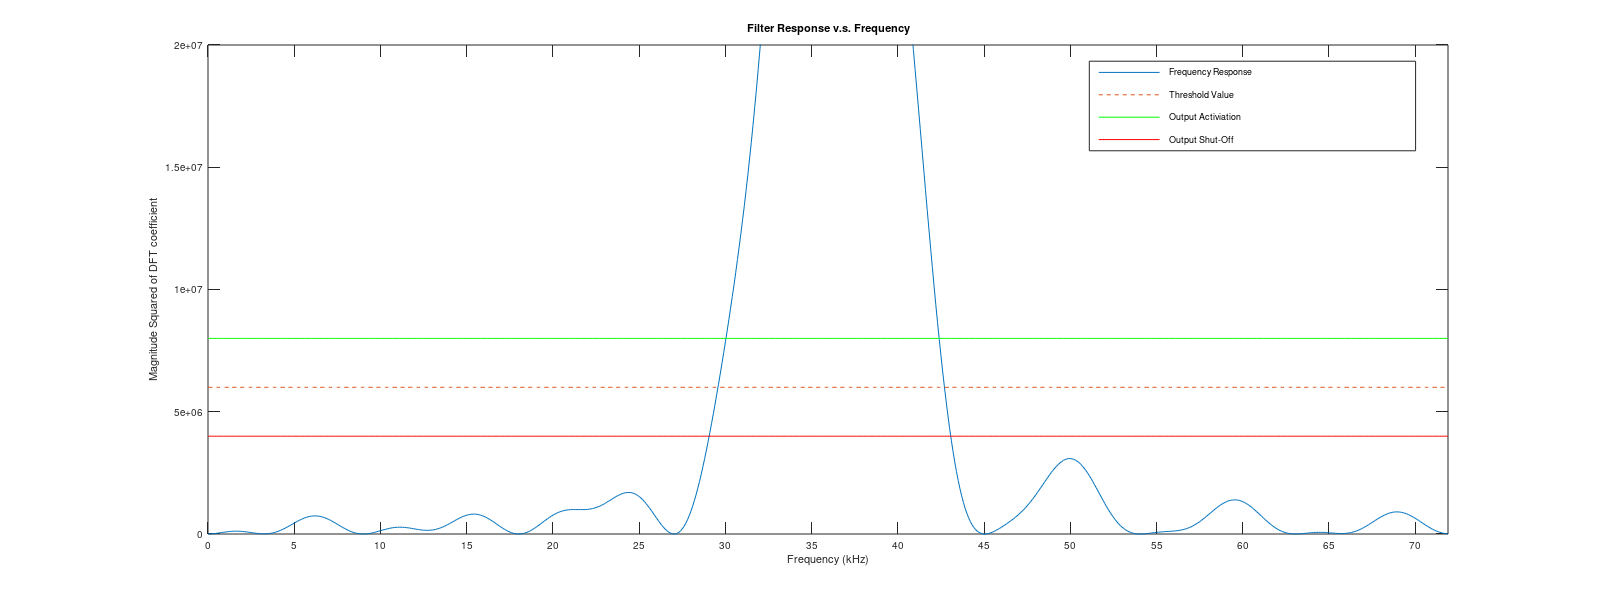
\includegraphics[width=.8\textwidth]{figures/design/schmit_simulation_wide.png}
	\caption{Schmitt Trigger Visualization}
	\label{fig:schmit_simulation_wide}
\end{figure}

Figure \ref{fig:schmit_simulation_wide} illustrates the Schmitt-trigger's activation and shut-off boundaries. The threshold and Schmitt-trigger values were chosen by inspecting the results from the frequency response experiment (see figure \ref{fig:goertzel_filter_response_simulated}) and selecting values which enable tone detection to work for signals of varying amplitudes.



%%%%%%%%%%%%%%%%%%%%%%%%%%%%%%%%%%%%%%%%%%%%%%%%%%%%%%%%%%%



\subsection{Tagger Software}

For this investigation, a tagger is created that can encode 16 bits of information. In this initial implementation, a single bit is reserved for error detection, however, further development of this system might explore the use of hamming codes which would require an additional four bits to be reserved for error correction.

\subsubsection{Modified RC-5 Protocol}
\label{sec:modified_rc5_protocol}
The RC-5 protocol is used as the basis for the transmission protocol. A detailed breakdown of the protocol is given in the literature review in section \ref{sec:rc_5_protocol}. In this modified version of the RC-5 protocol, the Manchester encoding technique and bit-period timing specifications are preserved. However, the structure of the bits transmitted is modified and the period between messages is decreased.

\begin{figure}[H]
	\centering
	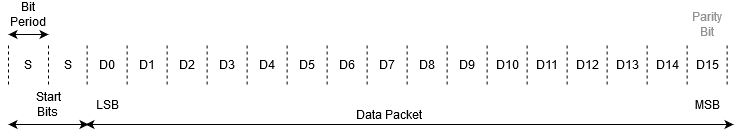
\includegraphics[width=0.8\linewidth]{figures/design/modified_rc5_protocol.png}
	\caption{Modified Bit Structure of RC-5 IR Protocol}
	\label{fig:modified_rc_5_protocol}
\end{figure}

Figure \ref{fig:modified_rc_5_protocol} shows the modified structure for a single transmission. The two start bits are preserved. The toggle bit, address bits and command bits are merged into a single set of data bits with an additional 4 bits added to increase the data packet size to 16 bits. In the modified protocol the bit order is reversed. It should be noted that data bit D15 is reserved for the parity checksum.

The original RC-5 protocol specifies a period of 114mS between transmissions. This period is longer than necessary and was reduced to 50mS based on the results recorded in section \ref{sec:processing_time_experiment}.

\subsubsection{Realization}

The tagger software comprises a set of functions dedicated to encoding a 15-bit data packet. The Manchester encoding is implemented using timers and interrupts to ensure precise timing and free the main processor for other tasks.

The following functions used in the generation of a Manchester waveform were created

\begin{lstlisting}[style=cstyle, caption=Transmission Related Functions\label{transmission_related_functions}]
uint8_t get_parity_15(uint16_t packet); //processes a 15-bit long data packet and returns the even parity
uint32_t wrap_data_15(uint16_t data); //processes a 15-bit long data packet and returns 18-bit bitstream for transmission
generate_manchester(uint32_t buffer, uint8_t num_bits); //starts Manchester encoded output generation on the pre-define GPIO based on the provided bitstream
\end{lstlisting}

%Using one of the dedicated timer peripherals (timer 17) and interrupts for the process of generating the Manchester encoded output required the use of global variables to track the status of an on-going transmission. The following listing shows the global variables along with a brief descriptor comment.

To track information between interrupt callback routines, a set of global variables are used. The code excerpt in listing \ref{lst:transmission_status_tracking_variables} shows these global variables and provides a brief description.

\begin{lstlisting}[style=cstyle, caption=Transmission Status Tracking Variables, label=lst:transmission_status_tracking_variables]
volatile uint32_t bit_stream; //bit-stream to be transmitted
volatile int bit_index; //index of bit currently being transmitted
volatile int bit_num_transmit; //number of bits from bit-stream to transmit
volatile int bit_period; //stores current bit period state (0 - first, 1 - second)
volatile int fire_in_progress; //global indicator of a transmission in progress
volatile int manchester_timeout_counter; //counts half bit-periods elapsed since last bit was transmitted
\end{lstlisting}

Interrupts and global variables open the possibility for data corruption. Although the STM32F0 is inherently a serial processor, the main-loop process (responsible for, among other things, initiating transmissions) and the transmission process share some properties with parallel processes. Figure \ref{fig:parallel_process_abstraction} illustrates how the operations performed during transmission can be abstracted as two parallel processes. It is necessary therefore, to provide a mechanism to prevent one process from modifying any of the shared variables (given in list \ref{lst:transmission_status_tracking_variables}) while the other is using them.

\begin{figure}[H]
	\centering
	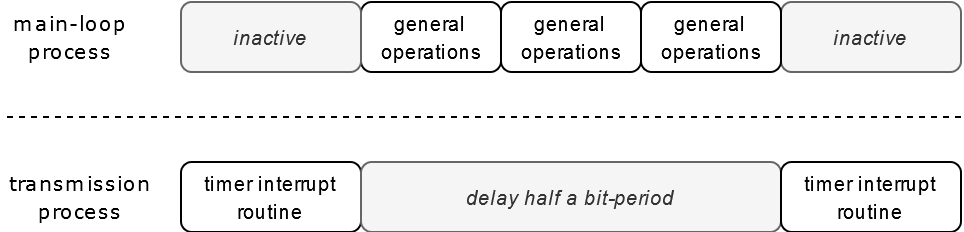
\includegraphics[width=0.8\linewidth]{figures/design/parallel_process_transmission.png}
	\caption{Parallel Process High-Level Abstraction}
	\label{fig:parallel_process_abstraction}
\end{figure}

The variable \textit{fire\_in\_progress} operates as a synchronization lock. As priority is given to the interrupt process, in the implementation of the function \textit{generate\_manchester} there is a loop which stalls the processor until any current transmissions complete, as indicated by this lock (see line 4, listing \ref{lst:generate_manchester_implementation}).

Finally, during the transmission process, the logic used to determine the pin state to generate the Manchester waveform is given in line 8 of listing \ref{lst:manchester_generate_interrupt_routine}. The pin state for each half bit-period is determined as follows: \[pin\_state = \overline{tx\_bit} \;\; \widehat{} \;\; bit\_period\] Where tx\_bit is the value of the bit currently being transmitted and bit\_period is as defined in listing \ref{lst:transmission_status_tracking_variables} above.




%%%%%%%%%%%%%%%%%%%%%%%%%%%%%%%%%%%%%%%%%%%%%%%%%%%%%%%%%%%


\subsection{Target Software}

In laser tag, it is optimal to have multiple IR detectors placed in various locations on the player. It is therefore important that the target software could be made capable of processing transmissions from multiple inputs simultaneously. This is achieved through the use of the input capture and output compare channels of the STM32's timer peripherals. For this investigation, the system is designed to monitor a single target, however, the process is easily expanded to capture signals from multiple targets.

The target MCU software was separated into four independent processes, these are outlined in figure \ref{fig:target_software_overview} below.

\begin{figure}[H]
	\centering
	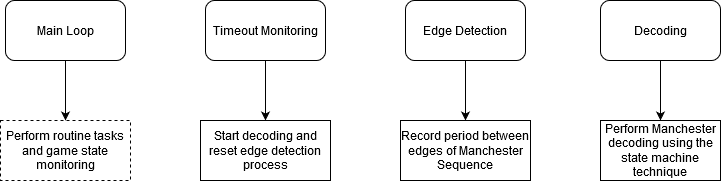
\includegraphics[width=0.8\linewidth]{figures/design/target_software_overview.png}
	\caption{Target MCU Processes}
	\label{fig:target_software_overview}
\end{figure}

The main loop process runs continually and may be used to perform routine tasks.

The edge detection process is an interrupt based process which monitors continuously for any rising or falling edges on the input GPIO pin. Each edge is recorded as a timestamp which measures the period elapsed since the previous edge was detected. To avoid performing unnecessary conversions, this value is stored as \textit{ticks} instead of seconds.

The timeout monitoring process is executed by an interrupt whenever the output compare register matches the timer's count value. Each time an edge is registered by the edge detection process, the output compare register value is adjusted to allow up to one timeout period before the interrupt is triggered.

The decoding process is also interrupt driven, however this process can also be triggered by software. A software trigger occurs when the maximum number of edges are recorded. The decoding process follows the state machine approach illustrated in figure \ref{fig:manchesterdecodingfsm} and uses the timestamps recorded by the edge detection process to decode incoming transmissions.

During the decoding process, the edge detection process is disabled.

\subsubsection{Decoding Strategy}

The state machine approach does not specify an end of transmission condition, therefore it is necessary to define one. It is not possible to simply count the number of bits received as the input capture stage and decoding stages operate independently. Therefore a timeout timer is used to trigger the decoding stage and reset the array of \textit{edge-time differences}. In addition to a timeout, if the maximum number of edges are recorded, the decoding process is automatically triggered by software.

%this needs more explaining but i cant...no time!!!
The timeout period is two bit-periods in duration. This is chosen because future inclusion of hamming codes would allow for the correction of a single flipped or missing bit. The timeout period of 3.556ms must be converted into ticks before being used by the output compare functionality of the timer.

\[TIMEOUT\_TICKS = f_{timer} \times T_{timeout} = 8 \times 10^6 \times 3.556 \times 10^{-3} = 28448\]

The maximum number of edges in a valid message occurs when all 16-bits are 1's which results in a Manchester sequence containing 36 edges. Therefore the edge detection process will automatically trigger the decoding process after 36 edges are recorded.

The implementation of the Manchester decoding algorithm may be found in the appendix, listing \ref{lst:decode_manchester_implementation}. Decoding requires the definition of a threshold duration to differentiate between long and short periods. This is the \textit{THRESHOLD\_TICKS} constant. A second constant \textit{BITMISS\_TICKS} is also defined, this threshold is used to detect when a bit in the received transmission goes undetected.








